% Retail world model paper: standalone two-column preprint.
% Compile with either engine, twice for refs/headers:
%   xelatex main.tex     (development; OpenType Pagella + Pagella Math)
%   pdflatex main.tex    (publisher compile services; Type 1 Pagella)
% Figures and tables are generated from the committed results by
%   make figures tables   (paper/Makefile)
\documentclass[10pt,twocolumn,letterpaper]{article}
\usepackage[letterpaper,margin=0.72in,columnsep=0.28in]{geometry}

% ---------------------------------------------------------------- fonts ---
% fontspec and unicode-math are XeTeX/LuaTeX only and abort under pdfTeX with
% "cannot-use-pdftex", which is what a pdfLaTeX-only submission system reports.
% tgpagella is the Type 1 build of the same typeface, so both engines set the
% document in Pagella and the pdfTeX path needs no other changes.
\usepackage{iftex}
\ifPDFTeX
  \usepackage[utf8]{inputenc}
  \usepackage[T1]{fontenc}
  \usepackage{tgpagella}
  \usepackage{textcomp}
  \usepackage{amssymb}          % \mathbb, which unicode-math supplies otherwise
\else
  \usepackage{fontspec}
  \usepackage{unicode-math}
  \setmainfont{TeX Gyre Pagella}
  % Pagella Math is preferred; Latin Modern Math is the documented fallback.
  \IfFontExistsTF{texgyrepagella-math.otf}
    {\setmathfont{TeX Gyre Pagella Math}}
    {\setmathfont{Latin Modern Math}}
\fi
\usepackage{newunicodechar}

% -------------------------------------------------------------- packages --
\usepackage{amsmath}
\usepackage{booktabs}
\usepackage{graphicx}
\usepackage{adjustbox}
\usepackage{rotating}
% Bounds for rotated floats. Inside a sidewaystable the page-geometry lengths
% are swapped, so these are derived from \paperwidth/\paperheight, which are
% not: after rotation a float may span the paper's height and is limited by the
% paper's width, less the margins and the caption.
\newlength{\rotmaxw}\setlength{\rotmaxw}{\dimexpr\paperheight-2in\relax}
\newlength{\rotmaxh}\setlength{\rotmaxh}{\dimexpr\paperwidth-3in\relax}
\usepackage[font=small,labelfont=bf,skip=6pt]{caption}
\usepackage{xcolor}
\usepackage[verbose=silent]{microtype}
\usepackage{titlesec}
\usepackage{fancyhdr}
\usepackage{pifont}

\definecolor{accent}{RGB}{38,78,120}
\definecolor{linkblue}{RGB}{20,60,110}
\definecolor{urlblue}{RGB}{0,84,166}
\definecolor{headtint}{RGB}{24,42,64}

\usepackage[colorlinks=true,
            linkcolor=linkblue,
            citecolor=linkblue,
            urlcolor=urlblue,
            filecolor=urlblue,
            breaklinks=true]{hyperref}

% ------------------------------------------------- unicode text fallbacks --
% Glyphs the text font does not carry, mapped so nothing is silently dropped,
% and mapped identically under both engines so the two builds agree.
%
% Under pdfTeX, inputenc already defines several of these (x, ->, +-, ^2, ^3,
% the middle dot, no-break space and non-breaking hyphen), so \newunicodechar
% emits "Redefining Unicode character" for each -- eight warnings a submission
% system reports back. The redefinitions are deliberate, so rather than
% silence the warning they go through inputenc's own supported override,
% \DeclareUnicodeCharacter, which does not warn. XeTeX has no inputenc and
% keeps \newunicodechar.
\ifPDFTeX
  \newcommand{\umap}[3]{\DeclareUnicodeCharacter{#2}{#3}}
\else
  \newcommand{\umap}[3]{\newunicodechar{#1}{#3}}
\fi
\umap{∈}{2208}{\ensuremath{\in}}
\umap{∉}{2209}{\ensuremath{\notin}}
\umap{∖}{2216}{\ensuremath{\setminus}}
\umap{∪}{222A}{\ensuremath{\cup}}
\umap{∩}{2229}{\ensuremath{\cap}}
\umap{⊆}{2286}{\ensuremath{\subseteq}}
\umap{⊂}{2282}{\ensuremath{\subset}}
\umap{ℝ}{211D}{\ensuremath{\mathbb{R}}}
\umap{∅}{2205}{\ensuremath{\emptyset}}
\umap{×}{00D7}{\ensuremath{\times}}
\umap{≤}{2264}{\ensuremath{\leq}}
\umap{≥}{2265}{\ensuremath{\geq}}
\umap{≈}{2248}{\ensuremath{\approx}}
\umap{≠}{2260}{\ensuremath{\neq}}
\umap{→}{2192}{\ensuremath{\rightarrow}}
\umap{↔}{2194}{\ensuremath{\leftrightarrow}}
\umap{−}{2212}{\ensuremath{-}}
\umap{±}{00B1}{\ensuremath{\pm}}
\umap{ρ}{03C1}{\ensuremath{\rho}}
\umap{τ}{03C4}{\ensuremath{\tau}}
\umap{Δ}{0394}{\ensuremath{\Delta}}
\umap{α}{03B1}{\ensuremath{\alpha}}
\umap{β}{03B2}{\ensuremath{\beta}}
\umap{²}{00B2}{\ensuremath{^{2}}}
\umap{³}{00B3}{\ensuremath{^{3}}}
\umap{₁}{2081}{\ensuremath{_{1}}}
\umap{₂}{2082}{\ensuremath{_{2}}}
\umap{·}{00B7}{\,\textperiodcentered\,}
\umap{✓}{2713}{\ding{51}}
\umap{✗}{2717}{\ding{55}}
\umap{ }{2009}{\,}   % U+2009 thin space
\umap{ }{00A0}{~}   % U+00A0 no-break space
\umap{‑}{2011}{-}   % U+2011 non-breaking hyphen

% ------------------------------------------------------------- spacing ----
\setlength{\parindent}{0pt}
\setlength{\parskip}{5.5pt plus 1.5pt}
\linespread{1.06}
\setlength{\textfloatsep}{12pt plus 3pt minus 3pt}
\setlength{\dbltextfloatsep}{14pt plus 3pt minus 3pt}
\setlength{\floatsep}{10pt plus 2pt minus 2pt}
\setlength{\intextsep}{10pt plus 2pt minus 2pt}
\renewcommand{\arraystretch}{1.3}

% Float economy: the default fractions push wide floats to the end of the
% document, which strands them in a block with no surrounding text. These
% let a page carry a large float *and* body text.
\renewcommand{\topfraction}{0.92}
\renewcommand{\dbltopfraction}{0.92}
\renewcommand{\bottomfraction}{0.5}
\renewcommand{\textfraction}{0.08}
\renewcommand{\floatpagefraction}{0.80}
\renewcommand{\dblfloatpagefraction}{0.80}
\setcounter{topnumber}{3}
\setcounter{dbltopnumber}{3}
\setcounter{totalnumber}{5}

\tolerance=1400
\emergencystretch=1.6em
\hbadness=3000

% ------------------------------------------------------------ headings ----
% Sections and subsections are numbered: the body cross-references them with
% \S\ref, which prints a bare "§" under secnumdepth 0.
\setcounter{secnumdepth}{2}
\newcommand{\secsquare}{%
  \textcolor{accent}{\rule[0.14em]{0.52em}{0.52em}}\hspace{0.42em}}
\titleformat{\section}
  {\normalfont\large\bfseries\color{headtint}}{\secsquare\thesection}{0.45em}{}
\titlespacing*{\section}{0pt}{16pt plus 4pt minus 2pt}{5pt plus 1pt}
\titleformat{\subsection}
  {\normalfont\normalsize\bfseries\color{headtint}}{\thesubsection}{0.45em}{}
\titlespacing*{\subsection}{0pt}{11pt plus 3pt minus 2pt}{3pt}
\titleformat{\paragraph}[runin]
  {\normalfont\bfseries\color{headtint}}{}{0pt}{}[.]
\titlespacing*{\paragraph}{0pt}{6pt plus 2pt}{0.6em}

% -------------------------------------------------------------- header ----
\newcommand{\shorttitle}{Forecasting for the grain the decision is made at}
\pagestyle{fancy}
\fancyhf{}
\fancyhead[L]{\footnotesize\textcolor{headtint}{\shorttitle}}
\fancyhead[R]{\footnotesize\thepage}
\renewcommand{\headrulewidth}{0.4pt}
\renewcommand{\headrule}{\hbox to\headwidth{\color{accent!45}\leaders\hrule height \headrulewidth\hfill}}
\setlength{\headheight}{18.7pt}\addtolength{\topmargin}{-6.7pt}

% ----------------------------------------------------- generated numbers --
% Generated by figs/make_tables.py from results/promoted and figs/rwdata.py. Do not edit.
\newcommand{\mWorldMarOverall}{0.642}
\newcommand{\mWorldMarTotal}{0.398}
\newcommand{\mWorldMarIxs}{0.851}
\newcommand{\mWorldMarFa}{0.991}
\newcommand{\mWorldMarSeeds}{3}
\newcommand{\mWorldMarOverallLo}{0.632}
\newcommand{\mWorldMarOverallHi}{0.648}
\newcommand{\mWorldMarIxsLo}{0.847}
\newcommand{\mWorldMarIxsHi}{0.853}
\newcommand{\mWorldAprOverall}{0.555}
\newcommand{\mWorldAprTotal}{0.283}
\newcommand{\mWorldAprIxs}{0.833}
\newcommand{\mWorldAprFa}{1.003}
\newcommand{\mWorldAprSeeds}{3}
\newcommand{\mWorldAprOverallLo}{0.550}
\newcommand{\mWorldAprOverallHi}{0.564}
\newcommand{\mWorldAprIxsLo}{0.831}
\newcommand{\mWorldAprIxsHi}{0.836}
\newcommand{\mWorldPracOverall}{0.656}
\newcommand{\mWorldPracTotal}{0.535}
\newcommand{\mWorldPracIxs}{0.834}
\newcommand{\mWorldPracFa}{0.952}
\newcommand{\mWorldPracSeeds}{3}
\newcommand{\mWorldPracOverallLo}{0.646}
\newcommand{\mWorldPracOverallHi}{0.675}
\newcommand{\mWorldPracIxsLo}{0.833}
\newcommand{\mWorldPracIxsHi}{0.835}
\newcommand{\mWorldTestOverall}{0.638}
\newcommand{\mWorldTestTotal}{0.379}
\newcommand{\mWorldTestIxs}{0.897}
\newcommand{\mWorldTestFa}{1.026}
\newcommand{\mWorldTestSeeds}{3}
\newcommand{\mWorldTestOverallLo}{0.627}
\newcommand{\mWorldTestOverallHi}{0.647}
\newcommand{\mWorldTestIxsLo}{0.896}
\newcommand{\mWorldTestIxsHi}{0.898}
\newcommand{\mLiftMarOverall}{0.664}
\newcommand{\mLiftMarTotal}{0.427}
\newcommand{\mLiftMarIxs}{0.846}
\newcommand{\mLiftMarFa}{0.966}
\newcommand{\mLiftMarSeeds}{3}
\newcommand{\mLiftMarOverallLo}{0.642}
\newcommand{\mLiftMarOverallHi}{0.680}
\newcommand{\mLiftMarIxsLo}{0.844}
\newcommand{\mLiftMarIxsHi}{0.847}
\newcommand{\mLiftAprOverall}{1.246}
\newcommand{\mLiftAprTotal}{0.964}
\newcommand{\mLiftAprIxs}{0.834}
\newcommand{\mLiftAprFa}{1.060}
\newcommand{\mLiftAprSeeds}{3}
\newcommand{\mLiftAprOverallLo}{0.566}
\newcommand{\mLiftAprOverallHi}{2.603}
\newcommand{\mLiftAprIxsLo}{0.832}
\newcommand{\mLiftAprIxsHi}{0.836}
\newcommand{\mLiftPracOverall}{0.713}
\newcommand{\mLiftPracTotal}{0.623}
\newcommand{\mLiftPracIxs}{0.832}
\newcommand{\mLiftPracFa}{0.941}
\newcommand{\mLiftPracSeeds}{3}
\newcommand{\mLiftPracOverallLo}{0.683}
\newcommand{\mLiftPracOverallHi}{0.734}
\newcommand{\mLiftPracIxsLo}{0.830}
\newcommand{\mLiftPracIxsHi}{0.833}
\newcommand{\mLiftTestOverall}{0.663}
\newcommand{\mLiftTestTotal}{0.368}
\newcommand{\mLiftTestIxs}{0.896}
\newcommand{\mLiftTestFa}{1.024}
\newcommand{\mLiftTestSeeds}{3}
\newcommand{\mLiftTestOverallLo}{0.622}
\newcommand{\mLiftTestOverallHi}{0.719}
\newcommand{\mLiftTestIxsLo}{0.895}
\newcommand{\mLiftTestIxsHi}{0.896}
\newcommand{\mLgbMarOverall}{0.709}
\newcommand{\mLgbMarTotal}{0.578}
\newcommand{\mLgbMarIxs}{0.873}
\newcommand{\mLgbMarFa}{0.943}
\newcommand{\mLgbMarSeeds}{3}
\newcommand{\mLgbMarOverallLo}{0.706}
\newcommand{\mLgbMarOverallHi}{0.713}
\newcommand{\mLgbMarIxsLo}{0.872}
\newcommand{\mLgbMarIxsHi}{0.874}
\newcommand{\mLgbAprOverall}{0.557}
\newcommand{\mLgbAprTotal}{0.351}
\newcommand{\mLgbAprIxs}{0.846}
\newcommand{\mLgbAprFa}{0.969}
\newcommand{\mLgbAprSeeds}{3}
\newcommand{\mLgbAprOverallLo}{0.551}
\newcommand{\mLgbAprOverallHi}{0.563}
\newcommand{\mLgbAprIxsLo}{0.845}
\newcommand{\mLgbAprIxsHi}{0.846}
\newcommand{\mLgbPracOverall}{0.715}
\newcommand{\mLgbPracTotal}{0.659}
\newcommand{\mLgbPracIxs}{0.847}
\newcommand{\mLgbPracSeeds}{1}
\newcommand{\mLgbTestOverall}{0.547}
\newcommand{\mLgbTestTotal}{0.247}
\newcommand{\mLgbTestIxs}{0.905}
\newcommand{\mLgbTestFa}{0.979}
\newcommand{\mLgbTestSeeds}{3}
\newcommand{\mLgbTestOverallLo}{0.547}
\newcommand{\mLgbTestOverallHi}{0.548}
\newcommand{\mLgbTestIxsLo}{0.905}
\newcommand{\mLgbTestIxsHi}{0.906}
\newcommand{\mGraphMarOverall}{0.778}
\newcommand{\mGraphMarTotal}{0.621}
\newcommand{\mGraphMarIxs}{0.878}
\newcommand{\mGraphMarFa}{1.058}
\newcommand{\mGraphMarSeeds}{3}
\newcommand{\mGraphMarOverallLo}{0.756}
\newcommand{\mGraphMarOverallHi}{0.815}
\newcommand{\mGraphMarIxsLo}{0.875}
\newcommand{\mGraphMarIxsHi}{0.881}
\newcommand{\mGraphAprOverall}{0.644}
\newcommand{\mGraphAprTotal}{0.493}
\newcommand{\mGraphAprIxs}{0.845}
\newcommand{\mGraphAprFa}{1.057}
\newcommand{\mGraphAprSeeds}{3}
\newcommand{\mGraphAprOverallLo}{0.627}
\newcommand{\mGraphAprOverallHi}{0.656}
\newcommand{\mGraphAprIxsLo}{0.844}
\newcommand{\mGraphAprIxsHi}{0.847}
\newcommand{\mGraphPracOverall}{0.641}
\newcommand{\mGraphPracTotal}{0.455}
\newcommand{\mGraphPracIxs}{0.851}
\newcommand{\mGraphPracFa}{0.962}
\newcommand{\mGraphPracSeeds}{3}
\newcommand{\mGraphPracOverallLo}{0.633}
\newcommand{\mGraphPracOverallHi}{0.654}
\newcommand{\mGraphPracIxsLo}{0.849}
\newcommand{\mGraphPracIxsHi}{0.853}
\newcommand{\mGraphTestOverall}{0.673}
\newcommand{\mGraphTestTotal}{0.412}
\newcommand{\mGraphTestIxs}{0.909}
\newcommand{\mGraphTestFa}{1.009}
\newcommand{\mGraphTestSeeds}{3}
\newcommand{\mGraphTestOverallLo}{0.669}
\newcommand{\mGraphTestOverallHi}{0.680}
\newcommand{\mGraphTestIxsLo}{0.907}
\newcommand{\mGraphTestIxsHi}{0.911}
\newcommand{\mTfmMarOverall}{0.854}
\newcommand{\mTfmMarTotal}{0.830}
\newcommand{\mTfmMarIxs}{0.836}
\newcommand{\mTfmMarFa}{0.920}
\newcommand{\mTfmMarSeeds}{1}
\newcommand{\mTfmAprOverall}{0.819}
\newcommand{\mTfmAprTotal}{0.786}
\newcommand{\mTfmAprIxs}{0.828}
\newcommand{\mTfmAprFa}{0.936}
\newcommand{\mTfmAprSeeds}{1}
\newcommand{\mTfmPracOverall}{0.896}
\newcommand{\mTfmPracTotal}{0.930}
\newcommand{\mTfmPracIxs}{0.828}
\newcommand{\mTfmPracFa}{0.904}
\newcommand{\mTfmPracSeeds}{1}
\newcommand{\mTfmTestOverall}{0.729}
\newcommand{\mTfmTestTotal}{0.558}
\newcommand{\mTfmTestIxs}{0.885}
\newcommand{\mTfmTestFa}{0.947}
\newcommand{\mTfmTestSeeds}{1}
\newcommand{\mNaiveMarOverall}{0.889}
\newcommand{\mNaiveMarTotal}{0.658}
\newcommand{\mNaiveMarIxs}{1.121}
\newcommand{\mNaiveMarFa}{0.940}
\newcommand{\mNaiveMarSeeds}{1}
\newcommand{\mNaiveAprOverall}{0.923}
\newcommand{\mNaiveAprTotal}{0.668}
\newcommand{\mNaiveAprIxs}{1.126}
\newcommand{\mNaiveAprFa}{0.971}
\newcommand{\mNaiveAprSeeds}{1}
\newcommand{\mNaivePracOverall}{0.870}
\newcommand{\mNaivePracTotal}{0.751}
\newcommand{\mNaivePracIxs}{1.100}
\newcommand{\mNaivePracSeeds}{1}
\newcommand{\mNaiveTestOverall}{0.847}
\newcommand{\mNaiveTestTotal}{0.560}
\newcommand{\mNaiveTestIxs}{1.176}
\newcommand{\mNaiveTestSeeds}{1}
\newcommand{\mTfmPlanMarOverall}{0.858}
\newcommand{\mTfmPlanMarIxs}{0.837}
\newcommand{\mTfmPlanAprOverall}{0.772}
\newcommand{\mTfmPlanAprIxs}{0.829}
\newcommand{\mTfmPlanPracOverall}{0.929}
\newcommand{\mTfmPlanPracIxs}{0.830}
\newcommand{\mTfmPlanTestOverall}{0.719}
\newcommand{\mTfmPlanTestIxs}{0.883}
\newcommand{\mLiftAprSeedAOverall}{0.566}
\newcommand{\mLiftAprSeedBOverall}{2.603}
\newcommand{\mLiftAprSeedCOverall}{0.570}
\newcommand{\mLiftAprSeedATotal}{0.270}
\newcommand{\mLiftAprSeedBTotal}{2.351}
\newcommand{\mLiftAprSeedCTotal}{0.271}
\newcommand{\fWorldFratOverall}{0.681}
\newcommand{\fWorldFratIxs}{0.665}
\newcommand{\fWorldFratFa}{1.000}
\newcommand{\fWorldFratOverallLo}{0.657}
\newcommand{\fWorldFratOverallHi}{0.702}
\newcommand{\fLgbFratOverall}{0.549}
\newcommand{\fLgbFratIxs}{0.608}
\newcommand{\fLgbFratFa}{0.937}
\newcommand{\fLgbFratOverallLo}{0.535}
\newcommand{\fLgbFratOverallHi}{0.561}
\newcommand{\fLiftFratOverall}{0.714}
\newcommand{\fLiftFratIxs}{0.677}
\newcommand{\fLiftFratFa}{0.977}
\newcommand{\fLiftFratOverallLo}{0.679}
\newcommand{\fLiftFratOverallHi}{0.744}
\newcommand{\fTfmFratOverall}{0.965}
\newcommand{\fTfmFratIxs}{0.827}
\newcommand{\fTfmFratFa}{0.847}
\newcommand{\fTfmPlanFratOverall}{0.686}
\newcommand{\fTfmPlanFratIxs}{0.641}
\newcommand{\fTfmPlanFratFa}{0.977}
\newcommand{\fWorldCheOverall}{0.897}
\newcommand{\fWorldCheIxs}{0.715}
\newcommand{\fWorldCheFa}{0.776}
\newcommand{\fWorldCheOverallLo}{0.881}
\newcommand{\fWorldCheOverallHi}{0.928}
\newcommand{\fWorldChePromo}{0.621}
\newcommand{\fWorldCheAfter}{0.952}
\newcommand{\fWorldCheOrdinary}{0.864}
\newcommand{\fLgbCheOverall}{0.708}
\newcommand{\fLgbCheIxs}{0.702}
\newcommand{\fLgbCheFa}{0.892}
\newcommand{\fLgbCheOverallLo}{0.699}
\newcommand{\fLgbCheOverallHi}{0.721}
\newcommand{\fLgbChePromo}{0.683}
\newcommand{\fLgbCheAfter}{1.173}
\newcommand{\fLgbCheOrdinary}{1.004}
\newcommand{\fTfmCheOverall}{0.829}
\newcommand{\fTfmCheIxs}{0.792}
\newcommand{\fTfmCheFa}{0.855}
\newcommand{\fTfmChePromo}{0.343}
\newcommand{\fTfmPlanCheOverall}{0.545}
\newcommand{\fTfmPlanCheIxs}{0.699}
\newcommand{\fTfmPlanChePromo}{0.685}
\newcommand{\fChePromoShare}{39}
\newcommand{\fWorldSnaOverall}{0.448}
\newcommand{\fWorldSnaIxs}{0.608}
\newcommand{\fWorldSnaFa}{0.929}
\newcommand{\fWorldSnaOverallLo}{0.397}
\newcommand{\fWorldSnaOverallHi}{0.531}
\newcommand{\fWorldSnaPromo}{0.882}
\newcommand{\fWorldSnaAfter}{0.958}
\newcommand{\fWorldSnaOrdinary}{0.951}
\newcommand{\fLgbSnaOverall}{0.412}
\newcommand{\fLgbSnaIxs}{0.596}
\newcommand{\fLgbSnaFa}{0.918}
\newcommand{\fLgbSnaOverallLo}{0.405}
\newcommand{\fLgbSnaOverallHi}{0.419}
\newcommand{\fLgbSnaPromo}{0.841}
\newcommand{\fLgbSnaAfter}{0.937}
\newcommand{\fLgbSnaOrdinary}{0.960}
\newcommand{\fTfmSnaOverall}{0.468}
\newcommand{\fTfmSnaIxs}{0.640}
\newcommand{\fTfmSnaFa}{0.927}
\newcommand{\fTfmSnaPromo}{0.630}
\newcommand{\fTfmPlanSnaOverall}{0.475}
\newcommand{\fTfmPlanSnaIxs}{0.614}
\newcommand{\fTfmPlanSnaPromo}{1.129}
\newcommand{\fSnaPromoShare}{34}
\newcommand{\fWorldSdrOverall}{0.830}
\newcommand{\fWorldSdrIxs}{0.734}
\newcommand{\fWorldSdrFa}{0.835}
\newcommand{\fWorldSdrOverallLo}{0.805}
\newcommand{\fWorldSdrOverallHi}{0.868}
\newcommand{\fWorldSdrPromo}{0.839}
\newcommand{\fWorldSdrAfter}{0.738}
\newcommand{\fWorldSdrOrdinary}{0.900}
\newcommand{\fLgbSdrOverall}{0.989}
\newcommand{\fLgbSdrIxs}{0.652}
\newcommand{\fLgbSdrFa}{0.743}
\newcommand{\fLgbSdrOverallLo}{0.982}
\newcommand{\fLgbSdrOverallHi}{0.996}
\newcommand{\fLgbSdrPromo}{0.759}
\newcommand{\fLgbSdrAfter}{0.585}
\newcommand{\fLgbSdrOrdinary}{0.824}
\newcommand{\fTfmSdrOverall}{1.070}
\newcommand{\fTfmSdrIxs}{0.895}
\newcommand{\fTfmSdrFa}{0.731}
\newcommand{\fTfmSdrPromo}{0.462}
\newcommand{\fTfmPlanSdrOverall}{0.974}
\newcommand{\fTfmPlanSdrIxs}{0.780}
\newcommand{\fTfmPlanSdrPromo}{0.932}
\newcommand{\fSdrPromoShare}{61}
\newcommand{\fWorldBjcOverall}{0.987}
\newcommand{\fWorldBjcIxs}{0.816}
\newcommand{\fWorldBjcFa}{0.839}
\newcommand{\fWorldBjcOverallLo}{0.943}
\newcommand{\fWorldBjcOverallHi}{1.029}
\newcommand{\fWorldBjcPromo}{0.477}
\newcommand{\fWorldBjcAfter}{0.881}
\newcommand{\fWorldBjcOrdinary}{0.921}
\newcommand{\fLgbBjcOverall}{0.994}
\newcommand{\fLgbBjcIxs}{0.750}
\newcommand{\fLgbBjcFa}{0.787}
\newcommand{\fLgbBjcOverallLo}{0.989}
\newcommand{\fLgbBjcOverallHi}{0.998}
\newcommand{\fLgbBjcPromo}{0.496}
\newcommand{\fLgbBjcAfter}{0.811}
\newcommand{\fLgbBjcOrdinary}{0.855}
\newcommand{\fTfmBjcOverall}{0.939}
\newcommand{\fTfmBjcIxs}{0.782}
\newcommand{\fTfmBjcFa}{0.866}
\newcommand{\fTfmBjcPromo}{0.327}
\newcommand{\fTfmPlanBjcOverall}{0.990}
\newcommand{\fTfmPlanBjcIxs}{0.754}
\newcommand{\fTfmPlanBjcPromo}{0.603}
\newcommand{\fBjcPromoShare}{18}
\newcommand{\fWorldAnaOverall}{0.867}
\newcommand{\fWorldAnaIxs}{0.713}
\newcommand{\fWorldAnaFa}{0.925}
\newcommand{\fWorldAnaOverallLo}{0.842}
\newcommand{\fWorldAnaOverallHi}{0.894}
\newcommand{\fWorldAnaPromo}{0.674}
\newcommand{\fWorldAnaAfter}{0.986}
\newcommand{\fWorldAnaOrdinary}{0.993}
\newcommand{\fLgbAnaOverall}{0.978}
\newcommand{\fLgbAnaIxs}{0.714}
\newcommand{\fLgbAnaFa}{0.904}
\newcommand{\fLgbAnaOverallLo}{0.970}
\newcommand{\fLgbAnaOverallHi}{0.987}
\newcommand{\fLgbAnaPromo}{0.648}
\newcommand{\fLgbAnaAfter}{0.939}
\newcommand{\fLgbAnaOrdinary}{0.977}
\newcommand{\fTfmAnaOverall}{1.008}
\newcommand{\fTfmAnaIxs}{0.790}
\newcommand{\fTfmAnaFa}{0.973}
\newcommand{\fTfmAnaPromo}{0.306}
\newcommand{\fTfmPlanAnaOverall}{0.889}
\newcommand{\fTfmPlanAnaIxs}{0.742}
\newcommand{\fTfmPlanAnaPromo}{0.779}
\newcommand{\fAnaPromoShare}{21}
\newcommand{\fWorldFreOverall}{0.485}
\newcommand{\fWorldFreIxs}{0.557}
\newcommand{\fWorldFreFa}{0.890}
\newcommand{\fWorldFreOverallLo}{0.476}
\newcommand{\fWorldFreOverallHi}{0.492}
\newcommand{\fWorldFrePromo}{0.800}
\newcommand{\fWorldFreAfter}{1.222}
\newcommand{\fWorldFreOrdinary}{0.914}
\newcommand{\fLgbFreOverall}{0.478}
\newcommand{\fLgbFreIxs}{0.529}
\newcommand{\fLgbFreFa}{0.795}
\newcommand{\fLgbFreOverallLo}{0.475}
\newcommand{\fLgbFreOverallHi}{0.483}
\newcommand{\fLgbFrePromo}{0.635}
\newcommand{\fLgbFreAfter}{1.088}
\newcommand{\fLgbFreOrdinary}{0.877}
\newcommand{\fTfmFreOverall}{0.563}
\newcommand{\fTfmFreIxs}{0.682}
\newcommand{\fTfmFreFa}{0.869}
\newcommand{\fTfmFrePromo}{0.290}
\newcommand{\fTfmPlanFreOverall}{0.566}
\newcommand{\fTfmPlanFreIxs}{0.599}
\newcommand{\fTfmPlanFrePromo}{0.942}
\newcommand{\fFrePromoShare}{40}
\newcommand{\promoTfmLo}{29}
\newcommand{\promoTfmHi}{63}
\newcommand{\promoTfmPlanLo}{60}
\newcommand{\promoTfmPlanHi}{113}
\newcommand{\promoWorldLo}{48}
\newcommand{\promoWorldHi}{88}
\newcommand{\promoLgbLo}{50}
\newcommand{\promoLgbHi}{84}
\newcommand{\promoShareLo}{18}
\newcommand{\promoShareHi}{61}
\newcommand{\tfmIxsGapWorldLo}{0.005}
\newcommand{\tfmIxsGapWorldHi}{0.014}
\newcommand{\tfmIxsGapLgbLo}{0.018}
\newcommand{\tfmIxsGapLgbHi}{0.037}
\newcommand{\tfmUnderLo}{5}
\newcommand{\tfmUnderHi}{10}
\newcommand{\worldVsTfmUpperLo}{21}
\newcommand{\worldVsTfmUpperHi}{47}
\newcommand{\cutSold}{120}
\newcommand{\cutWorld}{121, 600, 243}
\newcommand{\cutLift}{79, 206,886, 316}
\newcommand{\cutGraph}{59, 45, 55}
\newcommand{\cutLgb}{3.0, 3.0, 3.2}
\newcommand{\cutTfm}{7.8}
\newcommand{\liftSeedTwoForecast}{1,413,724}
\newcommand{\liftSeedTwoSold}{1,183,626}
\newcommand{\mPublishedWinner}{0.520}
\newcommand{\mPublishedTenth}{0.547}
\newcommand{\mPublishedFiftieth}{0.576}
\newcommand{\mPublishedStat}{0.671}
\newcommand{\nPromotedRuns}{110}
\newcommand{\computeHours}{44.7}
\newcommand{\computeRuns}{94}
\newcommand{\computeGpu}{Tesla T4}
\newcommand{\computeGpuMem}{14.6}
\newcommand{\computeCpu}{Intel Xeon CPU @ 2.00GHz}
\newcommand{\computeCores}{2}
\newcommand{\computeRam}{12.7}
\newcommand{\computeTorch}{2.11.0+cu130}
\newcommand{\computeCuda}{13.0}

\newcommand{\biasErrCorr}{0.87}
\newcommand{\biasErrN}{50}

\newcommand{\ixs}{item by store}

\begin{document}

% ------------------------------------------------------------ title block -
\twocolumn[
  \vspace*{6pt}
  \begin{center}
    {\LARGE\bfseries\color{headtint} Forecasting for the Grain the Decision Is Made At:\\[2pt]
     A Retail World Model on M5, Dominick's and Breakfast at the Frat\par}
    \vspace{10pt}
    {\large Karthik Iyer\par}
    \vspace{3pt}
    {\footnotesize Correspondence:
     \href{mailto:karthik.iyer488@gmail.com}{karthik.iyer488@gmail.com}
     \quad ORCID:
     \href{https://orcid.org/0009-0004-0593-1602}{0009-0004-0593-1602}\par}
    \vspace{18pt}
    \begin{minipage}{0.86\textwidth}
      \small
\textbf{Abstract.}
Which forecasting model is best depends on the level of the product and store
hierarchy at which the forecast is judged, and on how much of the sales the
plan (price, promotion, events) moves. We compare a world model, which carries
each item's state forward one period at a time under the plan, with a direct
lift model, LightGBM, a graph model, seasonal naive, and the pretrained
TimesFM~2.5 with and without the plan, on three public data sets: M5 (four
28-day windows), six Dominick's categories and Breakfast at the Frat. Every
model is scored at every level of the hierarchy, and every model and change
that lost is reported. On M5, TimesFM given only each item's sales history is
the most accurate model item by store in all four months
(\mTfmMarIxs{} to \mTfmTestIxs{}), but forecasts \tfmUnderLo\% to
\tfmUnderHi\% below total sales; the world model is the most accurate at the
chain total in two of the four months and LightGBM in one. The official M5 test
month is the only one of the four in which LightGBM is the most accurate over
all levels, so a single test month would have given the wrong ranking. On the
weekly, promotion-driven data, TimesFM without the plan forecasts
\promoTfmLo\% to \promoTfmHi\% of promoted-week sales and is behind both
plan-aware trained models item by store in six of seven data sets; given the
plan, it forecasts \promoTfmPlanLo\% to \promoTfmPlanHi\% and becomes the most
accurate model in one category. For an item whose first price cut in a year
sold \cutSold{} units, the world model forecast \cutWorld{} across three seeds,
against about 3 for LightGBM and 8 for TimesFM: plan-aware models respond in
the right direction, and the data do not fix the size. A retailer should
choose its forecasting model by the decision the forecast feeds, scored at
that decision's level and over several periods.

\vspace{4pt}
\textbf{Keywords:} retail forecasting; hierarchical evaluation; promotions;
world models; foundation models; M5.

    \end{minipage}
    \vspace{16pt}
  \end{center}
]
\thispagestyle{plain}

\section{Introduction}
\label{sec:intro}

A retailer uses sales forecasts for several decisions, and each decision is made
at its own grain of the product, store and time hierarchy. Store orders and
inventory are set for one item in one store, by day or week. Supplier funding
and deal terms are agreed for an item across all stores, by week. Category
performance is reviewed by category and store, week by week or over a run of
weeks, and category sales and margin plans are set for the category across the
chain. The financial plan is a chain total. A forecast can be accurate item by
store and still miss the category total by several percent, because small
errors in the same direction add up while large errors in opposite directions
cancel. Knowing which grain is being solved for therefore bears on which model
to use.

This paper asks that question directly: at which grain do which models
forecast best, when the price and promotion plan for the weeks ahead is known?
Of the four Ps of retail (product, price, promotion and place), it addresses
price and promotion, through the plan inputs that public data record: shelf
price, temporary price cuts, promotion flags, displays and circulars, event and
payment days. It does not forecast product (assortment, new items, ranging) or
place (space, distribution), and it does not solve the four together. A
forecast that did, or a retailer's own data with stock, space and range
recorded, could give different results from those reported here.

We compare models chosen to span what retailers use or are offered: LightGBM,
the tree model behind the leading M5 entries; the Temporal Fusion Transformer;
three pretrained models used without training on our data (TimesFM, Chronos-Bolt
and Timestral); a world model of our own, which turns each item's recent history
into a state and carries it forward one period at a time under the plan
(Figure~\ref{fig:overview}); the same network without the carried state; and an
equal-weight average of the world model, LightGBM and TimesFM given the plan.
An earlier version of this work scored one final window per data set and found
that the most accurate model changed with the level scored, the month and the
data set. This version tests that on rolling forecast origins taken before any
window used for development, on four public data sets, one of them kept out of
all development, with paired tests, model confidence sets, interval forecasts,
decision costs and reconciliation, every analysis written down before it ran
except checks of unexpected results and two corrections, which are marked where
they appear (Figure~\ref{fig:study}).

On these data sets, with the plan inputs and constraints they carry, we
observed the following.
\begin{enumerate}\setlength{\itemsep}{2pt}
\item \textbf{The model with the lowest error depended on the grain}
  (\S\ref{sec:res-grain}). For an item by store and an item across stores, the
  equal-weight average had the lowest error on \rgrain{ixs}{ens}{best} and
  \rgrain{item}{ens}{best} of nine data sets, and the 90\% confidence set kept
  few models with it (median \rgrain{ixs}{set}{median} and
  \rgrain{item}{set}{median} of nine). For a category by store, a category and
  the chain total, the lowest-error model differed from data set to data set
  and the confidence set kept a median of \rgrain{catstore}{set}{median}: with
  four to six windows, these data did not separate the models at these grains.
\item \textbf{The decision costs followed the same pattern.} For category-by-store
  plans the average had the lowest cost on \rcount{ccdollarsens} of eight data
  sets and LightGBM on \rcount{ccdollarslgb}, each ahead of the world model by an
  interval over category-by-store nodes that excludes zero (the world model was
  lower in at most two of the four to six windows); under the other horizon and
  weighting rules the lowest was the same kind of model with one exception. The
  world model was lowest only on M5, not separated by period and lower in all
  four windows over the whole window. A first version of
  this cost, which put the world model first on most data sets, was wrong
  (\S\ref{sec:res-decisions}). For store orders at critical ratios of 0.5 and
  0.8, the average or LightGBM had the lowest cost on every data set.
\item \textbf{LightGBM was the strongest single model at the fine grains, and
  averaging added to it.} LightGBM was more accurate than the world model item by
  store on \rcount{lgbbeatsworldixs} of eight data sets by the paired test. The
  average was more accurate than LightGBM item by store on
  \rcount{ensbeatslgbixs} and never less accurate. Weights fitted on earlier
  windows beat equal weights in \rcount{fittedwins} of \rcount{fittedn}
  comparisons (\S\ref{sec:res-ensemble}, \S\ref{sec:res-adds}).
\item \textbf{The world model added to the average on some data sets, and its
  carried state on almost none.} Without it the average was less accurate item
  by store on \rcount{withoutworldmodelixsens} data sets; on
  \rcount{addsnotliftixslist} we did not detect a difference when the same network
  without the carried state took its place, also on Frat when it was rerun with
  the world model's regularisation (\S\ref{sec:res-adds}, \S\ref{sec:res-world}).
\item \textbf{Every trained model used the plan, and pretrained models needed
  it.} Removing the plan inputs made every trained model less accurate; TimesFM
  with the plan was the most accurate model not trained on the data, and
  Timestral, released two days after this revision began, was behind it on
  every data set item by store and put extreme upper quantiles on a few weekly
  series (\S\ref{sec:res-plan}, \S\ref{sec:res-pretrained}).
\item \textbf{After a promotion the world model forecast more, not the dip that
  follows stocking up}, and the changes we tried for the dip were not kept
  (\S\ref{sec:res-plan}, \S\ref{sec:dropped}).
\item \textbf{Every model, test and change that lost is reported}, including a
  seed that never reached single-fit runs and run-to-run noise as large as the
  differences being tested (\S\ref{sec:dropped}).
\end{enumerate}

\begin{figure*}[t]
\centering
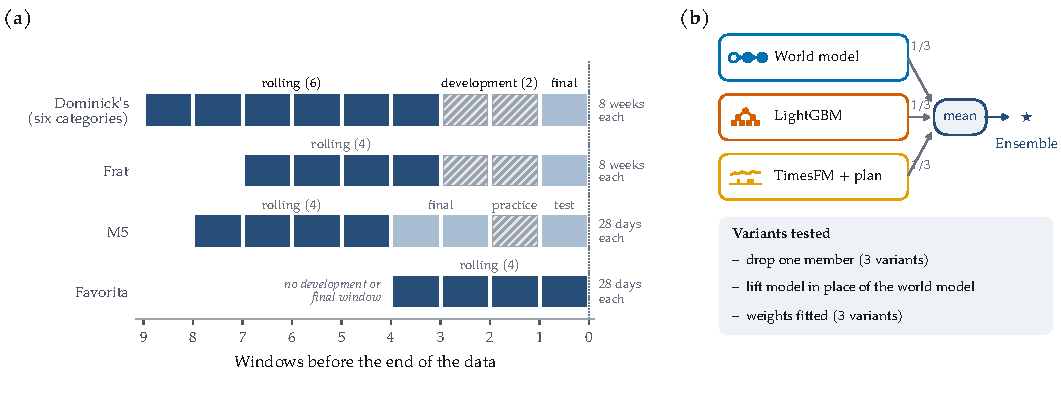
\includegraphics[width=\textwidth]{figs/fig_study.pdf}
\caption{\textbf{The main results come from rolling windows taken before any
window used to choose a setting, and the average tested is fixed in advance.} \textbf{(a)} Windows by data source, in periods before the end of the
data: rolling windows (scored for this revision), development windows (used to
choose settings) and final windows (scored once in the first version). Favorita
has rolling windows only; nothing was chosen on it. \textbf{(b)} The ensemble:
the equal-weight mean of the world model, LightGBM and TimesFM with the plan,
and the variants of study A that test what each member adds.}
\label{fig:study}
\end{figure*}

\begin{figure*}[t]
\centering
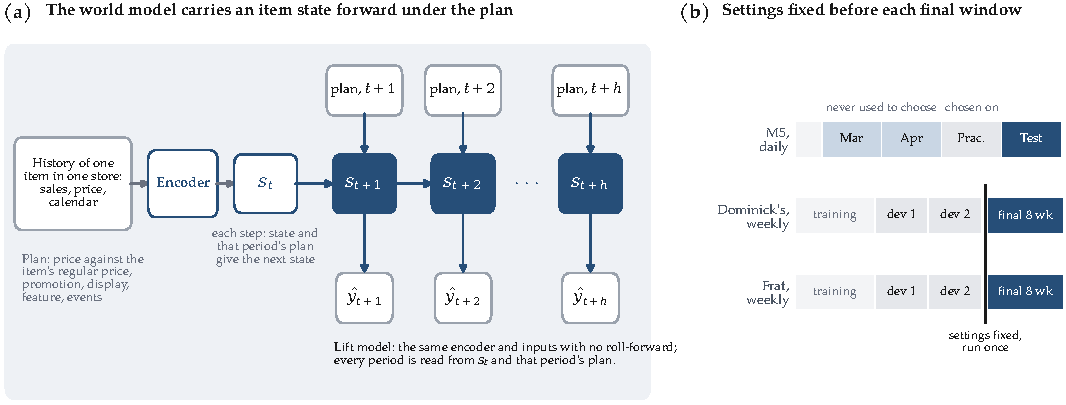
\includegraphics[width=\textwidth]{figs/fig_overview.pdf}
\caption{\textbf{The world model carries each item's state forward under the
plan.} \textbf{(a)} An encoder turns the recent history of one item in one store into
a state $s_t$. A transition step takes the state and one period's plan and
gives the state one period later; each period's sales are read from the state
as it stands after the plan so far. The lift model shares the encoder and
inputs and reads every period from $s_t$. \textbf{(b)} On M5, settings were
chosen on the practice window (25 April to 22 May 2016); on Dominick's and Frat,
on two development windows before the final 8 weeks.}
\label{fig:overview}
\end{figure*}

Section~\ref{sec:related} places the work among retail promotion models,
hierarchical evaluation, forecast combination, pretrained forecasters and world
models. Sections~\ref{sec:data} to \ref{sec:setup} give the data, the models and
the experimental setup. Section~\ref{sec:results} reports the results,
Section~\ref{sec:dropped} what was tried and dropped, and
Sections~\ref{sec:discussion} to \ref{sec:conclusion} discuss what the results
mean for a retailer, their limits, and conclude. The development study is in
Supplement~\ref{sec:supplementdev}, and the final windows and dropped changes of
the first version in Supplement~\ref{sec:supplementfinal}.

% =====================================================================
\section{Related work}
\label{sec:related}

\subsection{Retail forecasting and the promotion plan}

Fildes, Ma and Kolassa~\cite{fildes2022} review retail forecasting research and
practice and note that most studies forecast and evaluate at one level of
aggregation, usually the item, although retail decisions are spread across
levels. Sales of a single item in a single store are intermittent, which led to
dedicated methods for intermittent demand~\cite{croston,syntetos2005} and to
evaluating forecasts as count distributions~\cite{kolassa2016}. The Tweedie
family~\cite{jorgensen1987}, a compound Poisson--gamma distribution with a point
mass at zero, is the loss many M5 entries used, and the loss we use.

Promotions move retail sales more than anything else in the plan. PromoCast
forecast promoted-week sales for a chain from the planned event and the item's
past response~\cite{promocast}. Van Heerde, Leeflang and
Wittink~\cite{vanheerde2000} and Mac\'e and Neslin~\cite{mace2004} measured
the dips in sales before and after a promotion, when shoppers stock up and then
buy less. Ma, Fildes and Huang~\cite{ma2016} showed that promotional information
from within and across categories improves item-level forecasts.
Gupta~\cite{gupta1988} split the promotion bump into brand switching, purchase
timing and quantity, and van Heerde, Gupta and Wittink~\cite{vanheerde2003}
showed that in units only about a third of the bump is switching from other
brands. Attraction models make an item's sales the category's sales times its
share~\cite{bell1975,cooper1988}; our brand-switching step follows that
structure. Dominick's Finer Foods ran pricing experiments across its
stores~\cite{hoch1995}, and its scanner data are behind much of this
work~\cite{dominicks}.

\subsection{Hierarchies, combinations and evaluation}

Forecasts that must add up across a hierarchy are studied as hierarchical
forecasting, from bottom-up and top-down to optimal
reconciliation~\cite{athanasopoulos2009,hyndman2011,mint}. Our models forecast
item by store and their forecasts are summed, as the M5 accuracy competition
scored entries, with a weighted, scaled error averaged over twelve
levels~\cite{m5accuracy}; reconciliation is tested as a benchmark. The scaling
follows Hyndman and Koehler~\cite{hyndmankoehler}, and a companion competition
scored forecast distributions~\cite{m5uncertainty}. Tashman~\cite{tashman2000}
sets out why a comparison should use several forecast origins. Hansen, Lunde and
Nason's model confidence set~\cite{hansen2011} gives the set of models that
cannot be told apart from the best.

Combining forecasts from different models reduces error~\cite{batesgranger,clemen1989},
and an equal-weight average is hard to beat with estimated weights, the
forecast combination puzzle, which Smith and Wallis~\cite{smithwallis2009}
explain by the error in estimating the weights; Wang and
co-authors~\cite{wang2023} review the field. We fix an equal-weight ensemble in
advance and test weights fitted on earlier windows against it. Interval
forecasts by calibrating each model on its own past errors follow conformal
prediction~\cite{vovk2005}.

\subsection{Global models, trees and neural forecasters}

Global models, fitted across many series at once, are often more accurate than
one model per series~\cite{montero2021}. In M5 the leading entries were built on
gradient-boosted trees~\cite{lightgbm,januschowski2022}; the winner averaged
direct and recursive LightGBM models~\cite{inandjung}. Neural global models
include N-BEATS~\cite{nbeats}, DeepAR~\cite{deepar} and the Temporal Fusion
Transformer~\cite{tft}, the last two taking known future inputs such as price.
Graph neural networks share information between related
series~\cite{graphsage}; our item-to-item experiments use
attention~\cite{transformer} and conditional similarity
networks~\cite{veit2017}.

\subsection{Pretrained foundation models}

Pretrained time-series models forecast series they were not trained on.
TimesFM~\cite{timesfm} is a decoder-only transformer pretrained on a large
corpus of series; Chronos~\cite{chronos} tokenises values and trains a language
model on them, and Chronos-Bolt is its faster direct-quantile version;
Lag-Llama~\cite{lagllama}, Moirai~\cite{moirai} and TimeGPT~\cite{timegpt}
follow similar lines. TimesFM~2.5 adds a covariate method that fits a linear
model on future inputs and forecasts the remainder with the pretrained
model~\cite{timesfm25}. Timestral~1.0~\cite{timestral}, released by Mistral on
15 October 2026, reads known future inputs inside the model itself and returns
21 quantiles. We test whether any of them, given the plan, matches models
trained on it.

\subsection{World models and latent prediction}

A world model learns a state of its environment and how that state moves under
actions, so that the effect of a planned action can be rolled forward before it
is taken~\cite{worldmodels,planet,dreamerv3}. LeCun~\cite{lecun2022} proposed
joint-embedding predictive architectures (JEPA), which predict the
representation of the future rather than the future itself; I-JEPA~\cite{ijepa}
and V-JEPA~2~\cite{vjepa2} apply the idea to images and video, the latter with
an action-conditioned predictor used for planning. Such models guard against a
collapsed representation with a slowly updated target encoder~\cite{byol}, a
variance and covariance penalty~\cite{vicreg}, or the isotropic-Gaussian penalty
of LeJEPA~\cite{lejepa}, also used in LeWorldModel~\cite{leworldmodel}.
TD-MPC2~\cite{tdmpc2} rolls a latent state forward under actions; DWM~\cite{dwm}
keeps the effect of an action apart from the world's own dynamics, and
AD-WM~\cite{adwm} trains world models to tell actions apart for counterfactual
planning. Stable-worldmodel~\cite{stablewm} evaluates world models under
controlled changes, as our perturbation tests do. Closest to us,
WorldTS~\cite{worldts} learns covariate-conditioned latent dynamics for
forecasting with known future inputs. Our earlier work, M-JEPA~\cite{mjepa},
compared JEPA fine-tuning recipes with leakage-resistant splits. In retail the
actions are the plan. Our world model uses a recurrent transition~\cite{gru}
with layer normalisation~\cite{layernorm} on a transformer
encoder~\cite{transformer}, and is compared with the same model without the
transition so that what the carried state adds is measured on its own.

\subsection{What this paper adds}

Two findings here are not new. That an equal-weight average of different models
is hard to beat, and that fitted weights rarely help, is the forecast
combination puzzle~\cite{smithwallis2009,wang2023}; that a gradient-boosted tree
is a strong single model on retail panels was the lesson of M5~\cite{m5accuracy}.
Hierarchical forecasting asks how to make forecasts at different levels agree,
and scores them over all levels together~\cite{hyndman2011,mint,m5accuracy}. This
paper asks a different question: which model to choose for the grain at which a
given decision is made, when the price and promotion plan is known. It adds
three things to the work above. It scores each grain separately, ties each to
the decision made there, and reports how many models each grain's data can
separate, rather than one score averaged over levels; on these data the answer
differed between fine and coarse grains. It compares trained plan-aware models
with pretrained models given the plan as covariates on the same windows and
grains. And it measures, inside the average, what a model that carries a state
forward under the plan adds beyond the same network without it.

% =====================================================================
\section{Data}
\label{sec:data}

\begin{figure*}[t]
\centering
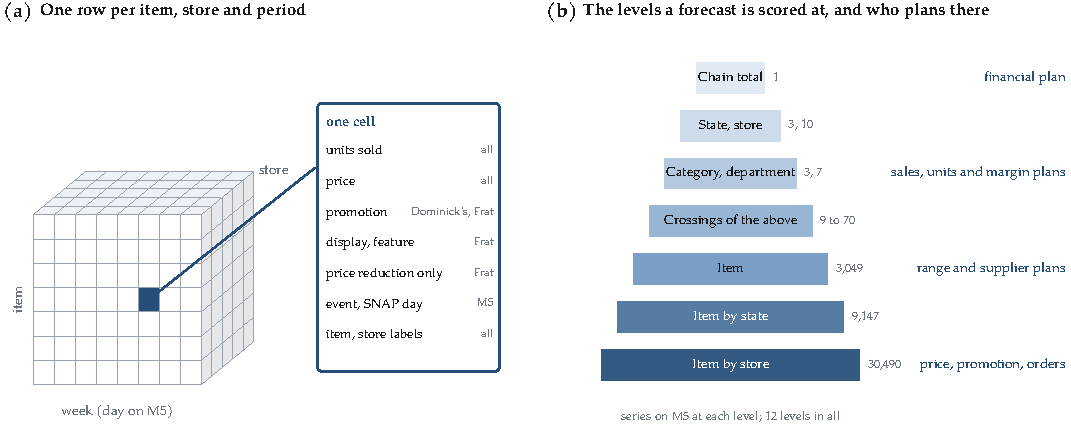
\includegraphics[width=\textwidth]{figs/fig_cube.pdf}
\caption{\textbf{Every data set is one table of item, store and period, scored
at every level a retailer plans at.} \textbf{(a)} Each cell holds the units sold,
the price and whatever plan the data set records; a lever a data set does not
record is passed to the models as unknown, not as zero. \textbf{(b)} The M5
hierarchy with the number of series at each level, and the decisions usually
made at each. Dominick's and Frat have six levels: total, category, store,
category by store, item and item by store; Favorita has total, store, family,
store by family, item and item by store.}
\label{fig:cube}
\end{figure*}

All four data sets are public (Table~\ref{tab:data}) and share one table shape
(Figure~\ref{fig:cube}a). \emph{M5} holds daily Walmart sales of 3,049 items in 10
stores across three states from 2011 to 2016, with prices by week, event days
and the days on which SNAP food assistance is paid~\cite{m5accuracy}.
\emph{Dominick's Finer Foods} holds weekly scanner data by store for a Chicago
chain from 1989 to 1997, with price, a promotion code and cost~\cite{dominicks}.
We use six categories chosen before any final run (cheese, snack crackers, soft
drinks, bottled juice, analgesics, frozen entrees). \emph{Breakfast at the Frat}
holds weekly sales of 55 breakfast items in 77 stores from 2009 to 2012, with
the shelf price, base price, and whether the item was on display, in the weekly
circular (feature) or on a tag-only price reduction~\cite{frat}.
\emph{Corporaci\'on Favorita} holds daily sales of an Ecuadorian grocery chain
to 15 August 2017~\cite{favorita}. It was added in this revision as a data set
kept out of development: the series are the 10 stores with the most units sold
in 2016 crossed with the items sold in all ten that year, from 1 January 2015;
returns are set to zero; the plan is the promotion flag, national holidays and
events, and paydays (the 15th and the last day of each month). Favorita records
no prices, so its WRMSSE weights are unit weights, not revenue weights. No raw
data is redistributed.

\begin{table}[t]
\centering
\caption{\textbf{Four public data sets, all scored item by store and at every
level above it.} Rolling windows were added in this revision and precede every
window used for development.}
\label{tab:data}
\footnotesize
\renewcommand{\arraystretch}{1.2}
\setlength{\tabcolsep}{4pt}
\begin{tabular}{p{0.17\columnwidth}p{0.14\columnwidth}p{0.27\columnwidth}p{0.28\columnwidth}}
\toprule
\textbf{Data} & \textbf{Series} & \textbf{Plan inputs} & \textbf{Rolling windows} \\
\midrule
M5 (daily) & 30,490 & Price, event days, SNAP days & Four of 28 days, Nov 2015 to Feb 2016 \\
Dominick's (weekly) & Six categories & Price, promotion & Six of 8 weeks per category \\
Frat (weekly) & 3,909 & Price, promotion, display, feature, price reduction only & Four of 8 weeks \\
Favorita (daily) & Top 10 stores & Promotion, holidays and events, paydays & Four of 28 days, the last ending 15 Aug 2017 \\
\bottomrule
\end{tabular}
\end{table}

\paragraph{Measure}
We use the weighted root mean squared scaled error (WRMSSE) of
M5~\cite{m5accuracy} at each level of the hierarchy: 12 levels on M5
(Figure~\ref{fig:cube}b) and six on the others. Each series' error is scaled by
its own in-sample one-step error, and series are weighted by their dollar sales
(units on Favorita) over the last weeks of training. We report item by store,
where orders and promotions are decided, the chain total, which a financial plan
is set against, and the mean over all levels (the M5 score). Lower is better.

% =====================================================================
\section{Models}
\label{sec:models}

Table~\ref{tab:models} lists every model. Each trained model's technique, loss
and settings are in this section and Table~\ref{tab:settings}; the constraints
each works within are in Appendix~\ref{sec:constraints}.

\begin{table}[t]
\centering
\caption{\textbf{Every forecast compared.} Plan: sees the plan for the
forecast periods. Trained: fitted on the data set. Timestral is also run from
history alone.}
\label{tab:models}
\footnotesize
\renewcommand{\arraystretch}{1.15}
\setlength{\tabcolsep}{3pt}
\begin{tabular}{p{0.33\columnwidth}ccp{0.38\columnwidth}}
\toprule
\textbf{Model} & \textbf{Plan} & \textbf{Trained} & \textbf{Technique and loss} \\
\midrule
Ensemble & yes & yes & Equal-weight mean of world model, LightGBM, TimesFM with the plan \\
World model & yes & yes & Item state rolled forward under the plan; Tweedie \\
Lift model & yes & yes & Same network, no roll-forward; Tweedie \\
LightGBM & yes & yes & Direct tree model per store; Tweedie \\
Temporal Fusion Transformer & yes & yes & Attention over history and plan; negative binomial \\
Graph model (M5 final only) & yes & yes & LightGBM's inputs with message passing; Tweedie \\
TimesFM with the plan & yes & no & TimesFM~2.5 with its covariate method \\
Timestral with the plan & yes & no & Timestral-28M with known future inputs \\
TimesFM & no & no & TimesFM~2.5, 512 periods of units \\
Chronos-Bolt & no & no & Chronos-Bolt base \\
Seasonal naive & no & no & Sales one season earlier \\
\bottomrule
\end{tabular}
\end{table}

\subsection{World model}

\paragraph{Encoder and state}
For item $i$ in one store, an encoder (a transformer over the last $L$
periods) reads sales and price, each scaled by the item's recent level
$\ell_i$, together with the calendar and the recorded levers, and gives a
state $s_t$; the item and store labels enter the readout. The item's level is
its average over the history window, or, on Dominick's, over its last 8 weeks.

\paragraph{Transition}
A gated recurrent transition $f$ carries the state forward under the plan
$p_{t+h}$ for each future period,
\begin{equation}
s_{t+h}(p) = \mathrm{LN}\big(f(p_{t+h},\, s_{t+h-1}(p))\big), \quad s_t(p) = s_t,
\end{equation}
where LN is layer normalisation (used on M5, Dominick's and Favorita). The plan
holds the period's price as a share of the item's regular price (its highest
price in the last 12 periods) and the recorded levers.

\paragraph{Readout and loss}
Expected sales are a baseline under the ``nothing planned'' plan $p^0$ (regular
price, no lever) times a lift,
\begin{equation}
\begin{split}
\log \mu_{i,t+h} = {} & \log \ell_i + b\big(s_{t+h}(p^0), p^0_{t+h}\big) \\
 & + g\big(s_{t+h}(p), p_{t+h}\big) - g\big(s_{t+h}(p^0), p^0_{t+h}\big),
\end{split}
\end{equation}
with $b$ and $g$ small networks that also take the item's labels and the
horizon step, and the log forecast bounded to $[-10, 10]$. The lift is exactly
zero when nothing is planned, and the baseline does not move when the plan
changes; both are checked by tests in the repository. Training minimises a
Tweedie loss on sales relative to $\ell_i$, with batches of item, store and
date drawn at random.

\paragraph{Brand switching (Dominick's)}
In a store and week where several items are promoted, much of each item's lift
is taken from the others. Following attraction models~\cite{bell1975,cooper1988},
the world model fits on the last 8 training weeks one number per run, the share
$\alpha$ of the summed lift that the category total keeps, and rescales its item
forecasts in each store and week so that the category total is the baseline
total plus $\alpha$ times the summed lift. $\alpha$ is a forecast-implied split
of lift, not an identified estimate of where promoted sales come from, because
promotions are not assigned at random. On Dominick's three fits with different
seeds are averaged in each run.

\begin{table}[t]
\centering
\caption{\textbf{The world model as run in the final tests.} Read from the run manifests in
\texttt{results/promoted/}. Periods are days on M5 and weeks on Dominick's and Frat.}
\label{tab:settings}
\footnotesize
\begin{tabular}{lrrr}
\toprule
\textbf{Setting} & \textbf{M5} & \textbf{Dominick's} & \textbf{Frat} \\
\midrule
Periods of history read & 112 & 26 & 26 \\
Periods of training data & 730 & 156 & 90 \\
State size & 128 & 64 & 64 \\
Encoder layers & 3 & 2 & 2 \\
Attention heads & 4 & 4 & 4 \\
Training steps & 30000 & 6000 & 3000 \\
Batch size & 1024 & 512 & 256 \\
Learning rate & 0.001 & 0.001 & 0.001 \\
Normalised roll-forward & yes & yes & no \\
Level from the last 8 weeks & no & yes & no \\
Brand switching & no & yes & no \\
Fits averaged per run & 1 & 3 & 1 \\
\bottomrule
\end{tabular}
\end{table}


\paragraph{What the state holds}
A probe on the frozen world model shows that the carried state takes in the
plan (Figure~\ref{fig:readback}): the day's discount can be read back from the
rolled state with $R^2$ 0.58 to 0.83 across three M5 windows, against $-0.01$ to
0.02 from the state before the window, and still at 0.46 to 0.59 seven days
later. That the plan is in the state does not show that the forecast uses it
well, which \S\ref{sec:res-plan} tests.

\begin{figure}[t]
\centering
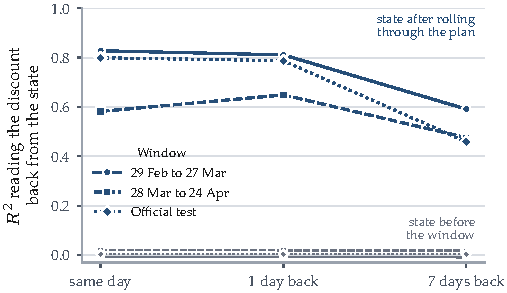
\includegraphics[width=\columnwidth]{figs/fig_readback.pdf}
\caption{\textbf{The rolled state holds the plan, and still holds most of it a
week later.} $R^2$ of a ridge read-out of the day's discount from the frozen
world model's state, fitted on half of 6,000 item-store pairs and scored on the
other half. Blue: the state after rolling through the window's plan. Grey: the
state before the window. Seed 1 in three M5 windows.}
\label{fig:readback}
\end{figure}

\subsection{Lift model}
The same model without the roll-forward: $s_{t+h}(p) = s_t$ for every $h$. On
M5, Dominick's and Favorita the two share encoder, readout, size, inputs, training
steps and regularisation, so the difference between them is the carried state; it
is the transition ablation. On Frat the lift model's settings, carried over from
the first version, add readout dropout~\cite{dropout} of 0.2 and decoupled weight
decay~\cite{adamw} of 0.01 that the world model does not use; study G reruns it
with the world model's settings (\S\ref{sec:res-adds}).

\subsection{Ensemble}
The equal-weight mean of the forecasts of the world model, LightGBM and TimesFM
with the plan for each item, store and period, fixed on 13 October 2026 before
any revision result, with no weights fitted. Its intervals come from its
own past errors like any other model's (\S\ref{sec:setup}).

\subsection{Comparison models}
\emph{LightGBM}~\cite{lightgbm}: one direct model per store, Tweedie loss,
sales at lags no shorter than the horizon, rolling averages and spread of
sales, price against the item's highest recent price, calendar and plan inputs.
\emph{Temporal Fusion Transformer}~\cite{tft}: one model per data set on
Dominick's and Frat, fitted on the last 156 weeks with the plan as known future
inputs and a negative binomial likelihood, 1,500 steps; it was not run on M5, where its
training cost was beyond the compute available, nor on Favorita, whose model
list was fixed without it. Chronos-Bolt and TimesFM from history alone were
not run on Favorita either. \emph{Graph model}: LightGBM's
inputs with one round of GraphSAGE-style message passing~\cite{graphsage}
between the same item in other stores and items of the same department in the
same store; run on the M5 final windows only. \emph{TimesFM}~\cite{timesfm,timesfm25}:
the 200M-parameter TimesFM~2.5 checkpoint given each series' last 512 periods;
we use its mean output, because its median forecasts 27\% to 31\% below M5
totals (\S\ref{sec:dropped-first}). \emph{TimesFM with the plan}: the same model
through its covariate method, a linear model on the plan inputs fitted over
groups of 2,048 series, then TimesFM on what that model leaves.
\emph{Chronos-Bolt}~\cite{chronos}: the base checkpoint, zero-shot, the mean of
its quantiles. \emph{Timestral}~\cite{timestral}: Timestral-28M (code commit
a534bdb), zero-shot, with the plan as known future inputs (price relative to
the context's highest price, other levers as given) and from history alone;
the point forecast is the mean of its 21 quantiles, each weighted by the share
of probability nearest it. \emph{Seasonal naive}: sales one season earlier.

% =====================================================================
\section{Experimental setup}
\label{sec:setup}

\paragraph{Windows}
On Dominick's and Frat the last 8 weeks of each data set were the final window
of the first version, touched once, and settings were chosen on the two 8-week
windows before it. On M5 settings were chosen on the practice window (25 April
to 22 May 2016), and the final windows were the official test month and, after
it, the two months before the practice window. For this revision each data set
gained rolling windows taken before the development windows, so none was used
for any choice: six 8-week windows on each Dominick's category, four on Frat,
and four 28-day windows on M5 (November 2015 to February 2016), each forecast
from everything earlier (Figure~\ref{fig:study}a). Favorita has four 28-day
rolling windows, the last ending on its last day, and no other.

\paragraph{Rules fixed in advance}
The revision plan, including every window, model, test and pass rule below,
was written down on 13 October 2026 before any revision run, and every change
to it is a dated amendment; all but the interval fix below were made before the
results they affect were read. Every
model runs in every rolling window with the settings of its final configuration,
unchanged. Trained models are one fit in the rolling windows: seed~1 where the
configuration names a seed (M5, Frat, LightGBM everywhere), and seed~0 for the
world model, lift model and TFT on Dominick's, whose configurations name none
and which, before a fix on 16 October, did not pass the run's seed to the model
(\S\ref{sec:dropped}). The final windows keep their three-seed results. No new result changes a setting of
a model already reported, and every model, window and test is reported.

\paragraph{Comparing two models}
For a window and a level, the difference in WRMSSE between two models gets a
95\% interval from 1,000 resamples of items: an item drawn twice counts twice in
every series and aggregate it feeds, with the weights recomputed. Across
windows, the mean difference gets a 95\% interval from 5,000 resamples of
windows. A model is said to beat another only when that interval excludes zero;
when it does not, we say no difference was detected, which is not a finding that
the two are equal. For each data set and level we report the 90\% model
confidence set~\cite{hansen2011} by the range statistic with a bootstrap over
windows. With four to six windows these tests have little power, and adjacent
windows are dependent: each is forecast from all data before it, so they share
most of their training history, and an error tied to a season or a stretch of
trading can recur in neighbouring windows. A bootstrap that resamples whole
windows treats them as exchangeable and so understates that dependence; we
report the number of windows in which one model beats another next to the
interval where it matters (\S\ref{sec:res-world}).

\paragraph{Intervals}
Each model's interval forecasts come from its own errors in the earlier rolling
windows of the same data set: errors scaled by each series' scale are pooled,
and their quantiles (2.5\% to 97.5\%) are added to the point forecast, a rolling
form of conformal calibration~\cite{vovk2005}. Where a level has fewer than 50
earlier errors for each horizon, all horizons are pooled into one set of
quantiles, and interval ends are rounded outwards to whole units except on
Favorita; this fix was added on 16 October after the first intervals covered
far less than planned at the totals, and both versions are reported. The first
rolling window has no earlier window and is not scored. We report the scaled
pinball loss averaged over the quantiles, weighted as in the M5 uncertainty
competition~\cite{m5uncertainty}, and coverage at 50\%, 80\% and 95\%. Models
that give quantiles of their own (Chronos-Bolt, TFT) are also scored on them,
over every window.

\paragraph{Decisions}
Three simulations turn forecasts into costs. \emph{Store orders}: for each
item-store-period, order the model's interval quantile at a critical ratio $r$
of 0.5, 0.8 or 0.95; each unit over costs 1 and each unit short $r/(1-r)$.
\emph{Category plan}: the absolute error of each category-by-store total in each
period, in dollars (each node's units valued at its average price before the
window), summed over the window and divided by sales in dollars; study G checks
it against the first half of the window, the error of the whole window's total,
units in place of dollars and equal node weights. \emph{Promotion decisions}: in the generated
store worlds of the companion paper~\cite{paper2}, where each promotion's true
lift is known, promote when the predicted lift times margin exceeds a fixed
cost; regret is the value lost against deciding with the true lift. The first
two are reported against seasonal naive. All are simulations under stated
costs, not business results.

\paragraph{Reconciliation}
Base forecasts at every node come from AutoETS fitted on the history before each
window (seasonal at the aggregate nodes, non-seasonal item by store). They are
reconciled bottom-up, top-down by historical proportions, and by the MinT
family~\cite{mint}: ordinary least squares, weighted least squares with
structural weights and with in-sample variances, and MinT with a shrunk
covariance where the hierarchy has at most 6,000 nodes (Frat); nodes with no
in-sample error are given the smallest variance of the others, a fix made after
the first run failed (\S\ref{sec:res-recon}). Each model's own
item-by-store forecasts are also combined with ETS above them by weighted least
squares.

\paragraph{Ranking}
Accuracy says how close a forecast is, not whether it puts items in the right
order. For every window we report the Spearman correlation, across item-store
series that sold in the window before, between the forecast change (horizon
total over the previous horizon's total) and the actual change; the share of the
tenth of nodes forecast to grow most that are in the actual top tenth (0.10 by
chance); the Spearman correlation across promoted periods between forecast and
actual units over the series' unpromoted level; and bias, forecast over actual.
These were written down before they ran and have no pass rule.

\paragraph{Studies added after the rolling results}
The rolling windows put the ensemble first, so studies were added, each
written down before it ran and reported as added after the main results:
\emph{A}, what each member adds to the ensemble and whether fitted weights beat
equal ones; \emph{B}, input perturbation on the saved models; \emph{C} and
\emph{E}, changes aimed at the forecast after a promotion; \emph{D}, Favorita;
\emph{F}, Timestral, with the ranking check alongside; and \emph{G}, asked for by
a reader of the first revision: paired uncertainty and sensitivity for the
category-plan cost, the Frat lift model rerun with the world model's
regularisation, and a diagnosis of the MinT failure. Study G found an error in
the category-plan cost and a numerical failure in MinT-shrink; both are
corrected and the first results kept for the record. Three tests on the
saved world models complete the set: shuffling the timing of the plan within
each series, adding one promotion and price cut and following its effect
through later periods, and a ridge read-out from the rolled state to sales after
the window.

% =====================================================================
\section{Results}
\label{sec:results}

All results in \S\ref{sec:res-ensemble} to \S\ref{sec:res-recon} are means over
the rolling windows; \S\ref{sec:res-final} gives the final windows of the first
version.

\subsection{The ensemble is the most accurate item-by-store forecast}
\label{sec:res-ensemble}

\begin{table*}[t]
\centering
\caption{\textbf{Over the rolling windows the equal-weight ensemble has the lowest item-by-store error on
\rcount{enslowestixs} of nine data sets, is in the 90\% model confidence set item by store on \rcount{ensinsetixs}
and at the total on \rcount{ensinsettotal}.} Mean WRMSSE over the rolling
windows (lower is better); W: windows. Bold: the lowest in the row. $^{\circ}$: in the 90\% model confidence set of
the row (Hansen, Lunde and Nason, range statistic, bootstrap over windows; Timestral, added in study F, is not
in the comparison). Ensemble: the equal-weight mean of the world model, LightGBM and TimesFM with the plan,
fixed before any rolling result. Neural models are one fit (seed~1). The Temporal Fusion Transformer was not run on M5
or Favorita, Chronos-Bolt, TimesFM and TFT not on Favorita. Timestral+plan is Timestral-28M with the plan (study F).}
\label{tab:rolling}
\footnotesize
\setlength{\tabcolsep}{3.4pt}
\begin{tabular}{lc*{10}{r}}
\toprule
\textbf{Data} & \textbf{W} & \rotatebox{70}{Ensemble} & \rotatebox{70}{World model} & \rotatebox{70}{Lift model} & \rotatebox{70}{LightGBM} & \rotatebox{70}{TimesFM+plan} & \rotatebox{70}{TimesFM} & \rotatebox{70}{Chronos-Bolt} & \rotatebox{70}{TFT} & \rotatebox{70}{Timestral+plan} & \rotatebox{70}{Seas.\ naive} \\
\midrule
\addlinespace[2pt]\multicolumn{12}{l}{\itshape Item by store} \\
Cheese & 6 & 0.934 & 1.713 & 1.119 & \textbf{0.623}$^{\circ}$ & 0.659 & 0.749 & 0.762 & 0.696 & 1.956 & 1.117 \\
Snack crackers & 6 & \textbf{0.562}$^{\circ}$ & 0.595 & 0.598 & 0.578 & 0.605 & 0.677 & 0.708 & 0.654 & 1.944 & 1.010 \\
Soft drinks & 6 & \textbf{0.536}$^{\circ}$ & 0.600 & 0.672 & 0.545$^{\circ}$ & 0.609 & 0.711 & 0.720 & 0.640 & 0.872 & 0.960 \\
Bottled juice & 6 & \textbf{0.585}$^{\circ}$ & 0.656 & 0.616 & 0.605 & 0.636 & 0.712 & 0.728 & 0.676 & 1.459 & 1.079 \\
Analgesics & 6 & 0.650$^{\circ}$ & 0.672 & 0.677 & \textbf{0.647}$^{\circ}$ & 0.679 & 0.734 & 0.745 & 0.693 & 2.111 & 0.997 \\
Frozen entrees & 6 & \textbf{0.408}$^{\circ}$ & 0.433 & 0.449 & 0.410$^{\circ}$ & 0.487 & 0.549 & 0.554 & 0.488 & 1.048 & 0.710 \\
Frat & 4 & \textbf{0.549}$^{\circ}$ & 0.595 & 0.590 & 0.570 & 0.578 & 0.775 & 0.778 & 0.652 & 0.864 & 1.077 \\
M5 & 4 & \textbf{0.834}$^{\circ}$ & 0.851 & 0.845 & 0.861 & 0.842 & 0.842 & 0.858 & -- & 0.894 & 1.163 \\
Favorita & 4 & \textbf{0.694}$^{\circ}$ & 0.726 & 0.744 & 0.719 & 0.712 & -- & -- & -- & 0.731 & 0.992 \\
\addlinespace[2pt]\multicolumn{12}{l}{\itshape Total} \\
Cheese & 6 & \textbf{0.371}$^{\circ}$ & 0.585$^{\circ}$ & 0.617$^{\circ}$ & 0.456$^{\circ}$ & 0.584 & 0.718 & 0.790 & 0.481$^{\circ}$ & 4.606 & 1.175 \\
Snack crackers & 6 & 1.181$^{\circ}$ & 1.454$^{\circ}$ & \textbf{1.026}$^{\circ}$ & 1.097$^{\circ}$ & 1.181$^{\circ}$ & 1.581$^{\circ}$ & 4.410$^{\circ}$ & 1.301$^{\circ}$ & 16.272 & 1.790$^{\circ}$ \\
Soft drinks & 6 & 0.834$^{\circ}$ & 0.879$^{\circ}$ & 0.965$^{\circ}$ & \textbf{0.831}$^{\circ}$ & 0.977 & 1.157 & 1.270 & 0.971 & 4.181 & 1.035 \\
Bottled juice & 6 & \textbf{0.525}$^{\circ}$ & 0.613$^{\circ}$ & 0.585$^{\circ}$ & 0.530$^{\circ}$ & 0.766$^{\circ}$ & 0.898 & 0.897 & 0.793 & 6.257 & 1.390 \\
Analgesics & 6 & \textbf{0.782}$^{\circ}$ & 0.826$^{\circ}$ & 0.868$^{\circ}$ & 0.869$^{\circ}$ & 0.848$^{\circ}$ & 0.900$^{\circ}$ & 0.979 & 1.057$^{\circ}$ & 31.256 & 1.796 \\
Frozen entrees & 6 & 0.342$^{\circ}$ & 0.338$^{\circ}$ & 0.387$^{\circ}$ & \textbf{0.321}$^{\circ}$ & 0.481 & 0.500 & 0.578 & 0.380 & 2.158 & 0.620 \\
Frat & 4 & 0.337$^{\circ}$ & 0.457 & 0.405$^{\circ}$ & 0.360$^{\circ}$ & \textbf{0.327}$^{\circ}$ & 0.541 & 0.605 & 0.425 & 1.048 & 0.964 \\
M5 & 4 & 0.706$^{\circ}$ & \textbf{0.609}$^{\circ}$ & 1.163$^{\circ}$ & 0.693$^{\circ}$ & 1.035 & 1.000 & 1.333 & -- & 1.025 & 1.087 \\
Favorita & 4 & \textbf{0.303}$^{\circ}$ & 0.341$^{\circ}$ & 0.452 & 0.309$^{\circ}$ & 0.397 & -- & -- & -- & 0.403 & 0.501 \\
\bottomrule
\end{tabular}
\end{table*}


\begin{figure*}[t]
\centering
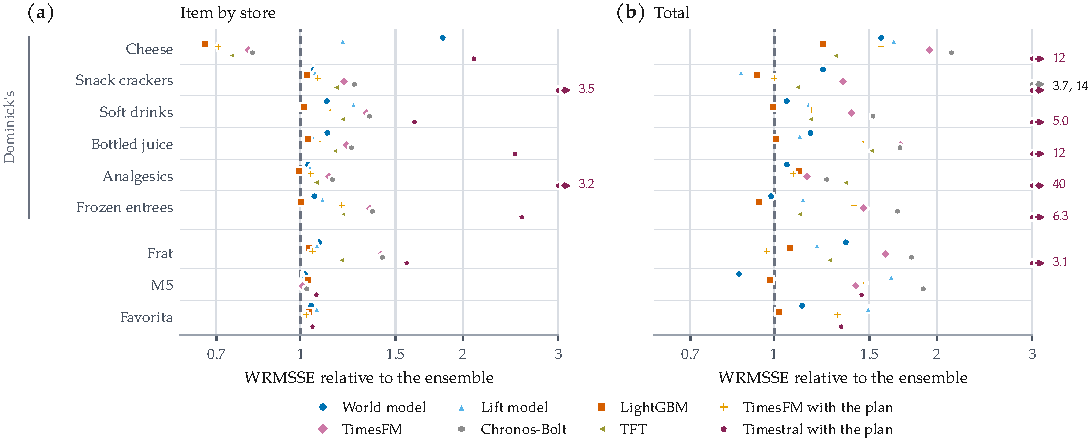
\includegraphics[width=\textwidth]{figs/fig_rolling.pdf}
\caption{\textbf{Item by store, every single model is less accurate than the
ensemble on almost every data set; at the total the ensemble is never far from
the best and the best single model changes with the data set.} Mean WRMSSE over
the rolling windows of each model divided by the ensemble's (dashed line at 1;
log scale; left of the line is more accurate than the ensemble).
\textbf{(a)} Item by store. \textbf{(b)} Chain total. Values beyond the axis are
marked at its edge with their value. Six, four, four and four windows on
Dominick's, Frat, M5 and Favorita.}
\label{fig:rolling}
\end{figure*}

The equal-weight ensemble has the lowest item-by-store error on
\rcount{enslowestixs} of the nine data sets (Table~\ref{tab:rolling},
Figure~\ref{fig:rolling}a). In the other two, analgesics and cheese, LightGBM
is lower: \rv{ana}{lgb}{ixs} against \rv{ana}{ens}{ixs} in analgesics, where
both are in the model confidence set, and \rv{che}{lgb}{ixs} against
\rv{che}{ens}{ixs} in cheese, the one data set where LightGBM is alone in the
set. The ensemble is in the 90\% model confidence set item by store on
\rcount{ensinsetixs} data sets and alone in it on
\rcount{ensaloneixs} (\rcount{ensaloneixslist}). At the chain total it is in
the set on all \rcount{ensinsettotal}, and it has the lowest error on
\rcount{enslowesttotal}; elsewhere the lowest belongs to
\rcount{lowesttotallist}.

By the paired test over windows, the ensemble is more accurate than LightGBM
item by store on \rcount{ensbeatslgbixs} of the eight data sets with paired
results (\rcount{ensbeatslgbixslist}; M5: \rv{mfive}{ens}{ixs} against
\rv{mfive}{lgb}{ixs}) and at the total on \rcount{ensbeatslgbtotal}
(\rcount{ensbeatslgbtotallist}). It is more accurate than the world model item
by store on \rcount{ensbeatsworldixs} and at the total on
\rcount{ensbeatsworldtotal} (\rcount{ensbeatsworldtotallist}). It is less
accurate than either at either level on none. The Temporal Fusion Transformer,
Chronos-Bolt and TimesFM from history alone are behind the ensemble item by store
on every data set where they ran.

The cheese result comes from one window. In one of the six cheese windows the
world model's item-by-store WRMSSE was \rwin{che}{world}{ixsmax}, against a
median of \rwin{che}{world}{ixsmedian} over the six, and the lift model's
\rwin{che}{lift}{ixsmax}; the ensemble, a third of whose forecast is the world
model's, inherits part of that error.

\subsection{What the world model adds to the ensemble}
\label{sec:res-adds}

\begin{table*}[t]
\centering
\caption{\textbf{Removing the world model makes the ensemble less accurate item by store on \rcount{withoutworldmodelixsens}
data sets and at the total on \rcount{withoutworldmodeltotalens}; replacing it with the lift model, the same network
without the carried state, does so on \rcount{liftforworldmodelixsens} and \rcount{liftforworldmodeltotalens}.}
Mean WRMSSE of each variant minus the ensemble's over the rolling windows (study A, added after the rolling results);
above zero the ensemble is more accurate. Bold: the ensemble is more accurate and the 95\% interval from the bootstrap
over windows excludes zero; underlined: the variant is, with the same test. No X: the equal-weight mean of the other two
members ($-$World: without the world model; $-$LGB: without LightGBM; $-$TFM+p: without TimesFM with the plan). Lift:
the world model replaced by the lift model. Fitted: weights chosen on the earlier
windows of the data set (lowest mean WRMSSE over all levels), scored on the next, so one window fewer.}
\label{tab:ablation}
\footnotesize
\setlength{\tabcolsep}{3.2pt}
\begin{tabular}{l*{10}{r}}
\toprule
 & \multicolumn{5}{c}{\textbf{Item by store}} & \multicolumn{5}{c}{\textbf{Total}} \\
\cmidrule(lr){2-6}\cmidrule(lr){7-11}
\textbf{Data} & $-$World & $-$LGB & $-$TFM+p & Lift & Fitted & $-$World & $-$LGB & $-$TFM+p & Lift & Fitted \\
\midrule
Cheese & \textminus 0.328 & \textbf{0.199} & \textbf{0.190} & \textminus 0.196 & \textbf{0.015} & 0.072 & \textbf{0.056} & 0.029 & 0.021 & 0.056 \\
Snack crackers & 0.002 & \textbf{0.018} & 0.004 & 0.002 & 0.004 & \textminus 0.095 & 0.118 & 0.013 & \textminus 0.145 & \textminus 0.073 \\
Soft drinks & 0.008 & \textbf{0.023} & 0.009 & \textbf{0.015} & \textminus 0.006 & 0.025 & \textbf{0.045} & \textminus 0.022 & \textminus 0.007 & \textminus 0.008 \\
Bottled juice & \textbf{0.012} & \textbf{0.016} & \textbf{0.015} & 0.002 & 0.000 & \textbf{0.103} & 0.031 & \textminus 0.042 & 0.051 & \textminus 0.015 \\
Analgesics & 0.000 & \textbf{0.014} & \textminus 0.001 & \textbf{0.003} & \textbf{0.008} & 0.019 & \textminus 0.006 & 0.038 & \textbf{0.025} & 0.012 \\
Frozen entrees & \textbf{0.012} & \textbf{0.019} & \textminus 0.002 & 0.005 & \textminus 0.001 & \textbf{0.025} & \textbf{0.034} & \textminus 0.026 & 0.013 & \textminus 0.015 \\
Frat & 0.002 & \textbf{0.010} & \textbf{0.012} & 0.001 & \textbf{0.007} & \underline{\textminus 0.040} & \textbf{0.021} & \textbf{0.051} & \textminus 0.017 & \underline{\textminus 0.022} \\
M5 & \textbf{0.005} & 0.003 & \textbf{0.006} & \textminus 0.001 & \textbf{0.013} & \textbf{0.113} & 0.050 & \underline{\textminus 0.112} & 0.000 & \textminus 0.037 \\
Favorita & \textbf{0.007} & \textbf{0.006} & \textbf{0.007} & \textbf{0.010} & \textbf{0.007} & 0.037 & 0.013 & \underline{\textminus 0.015} & \textbf{0.067} & 0.004 \\
\bottomrule
\end{tabular}
\end{table*}


\begin{figure*}[t]
\centering
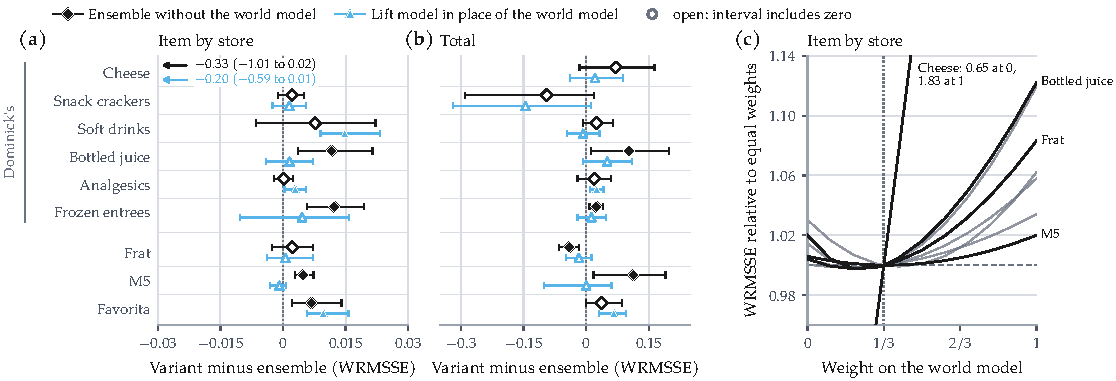
\includegraphics[width=\textwidth]{figs/fig_ablation.pdf}
\caption{\textbf{Taking the world model out of the ensemble costs accuracy on
some data sets; replacing it with the same network without the carried state
costs less often.} \textbf{(a, b)} Mean WRMSSE of the ensemble without the
world model, and with the lift model in its place, minus the ensemble's, with
95\% intervals from the bootstrap over windows; right of zero the ensemble with
the world model is more accurate; filled markers: the interval excludes zero.
\textbf{(a)} Item by store. \textbf{(b)} Total. \textbf{(c)} Item by store:
the ensemble's WRMSSE as the world model's weight goes from 0 to 1 (the other
two sharing the rest equally), relative to equal weights (dotted line at
one third), one line per data set. Study A, saved forecasts only.}
\label{fig:ablation}
\end{figure*}

Each member earns its place on some data sets and none on all
(Table~\ref{tab:ablation}). Without the world model the ensemble is less
accurate item by store on \rcount{withoutworldmodelixsens}
(\rcount{withoutworldmodelixsenslist}) and at the total on
\rcount{withoutworldmodeltotalens} (\rcount{withoutworldmodeltotalenslist}); on
Frat at the total it is more accurate without it
(\rab{frat}{withoutworldmodel}{total}{meandiff}). Without LightGBM it is less
accurate item by store on \rcount{withoutlightgbmixsens} and at the total on
\rcount{withoutlightgbmtotalens}. Without TimesFM with the plan it is less
accurate item by store on \rcount{withouttimesfmixsens}, at the total on
\rcount{withouttimesfmtotalens}, and more accurate at the total on
\rcount{withouttimesfmtotalvar} (\rcount{withouttimesfmtotalvarlist}).
LightGBM is the member the ensemble can least do without.

Some of the world model's contribution is any third model's. With the lift
model in its place, which has the same encoder, readout, inputs and training and
no carried state, the ensemble is less accurate item by store on
\rcount{liftforworldmodelixsens} data sets (\rcount{liftforworldmodelixsenslist})
and at the total on \rcount{liftforworldmodeltotalens}
(\rcount{liftforworldmodeltotalenslist}), and more accurate on none. The carried
state therefore adds to the ensemble where those intervals exclude zero, and
elsewhere the gain from the world model is a gain from adding a third,
different model.

Equal weights are hard to beat. Weights chosen on the earlier windows of each
data set, for item by store, for the total or for all levels, and scored on the
next window, are more accurate than equal weights in \rcount{fittedwins} of
\rcount{fittedn} comparisons and less accurate in \rcount{fittedlosses}. The
fitted weights do say where each member is useful: chosen for the total, the
world model's mean weight is \rw{ana}{total}{world} in analgesics and
\rw{mfive}{total}{world} on M5, against \rw{ana}{bottom}{world} and
\rw{mfive}{bottom}{world} chosen for item by store. Figure~\ref{fig:ablation}c
shows the item-by-store error is flat across a wide range of the world model's
weight on most data sets, which is why fitting the weights gains little.

\subsection{The world model on its own}
\label{sec:res-world}

On its own the world model is behind LightGBM item by store and level with it
at the total. By the paired test LightGBM is more accurate item by store on
\rcount{lgbbeatsworldixs} of eight data sets (\rcount{lgbbeatsworldixslist})
and at the total on \rcount{lgbbeatsworldtotal} (\rcount{lgbbeatsworldtotallist});
the world model is more accurate than LightGBM on \rcount{worldbeatslgbixs} at
either level. Its lowest error is at the M5 chain total,
\rv{mfive}{world}{total} against \rv{mfive}{lgb}{total} for LightGBM and
\rv{mfive}{ens}{total} for the ensemble, but the windows differ enough that
the difference is not outside its interval (LightGBM minus the world model
\rpair{mfive}{lgb}{world}{total}{meandiff}, interval
\rpair{mfive}{lgb}{world}{total}{lo} to \rpair{mfive}{lgb}{world}{total}{hi}).

Against the lift model, which differs only in the carried state, the world model
is more accurate item by store on \rcount{worldbeatsliftixs}
(\rcount{worldbeatsliftixslist}), less accurate on \rcount{liftbeatsworldixs}
(\rcount{liftbeatsworldixslist}), and level at the total on all eight. Taken
alone, carrying the state forward neither helps nor hurts accuracy in most data
sets. Its value shows in what it adds to the ensemble (\S\ref{sec:res-adds}) and
in category plans (\S\ref{sec:res-decisions}), where the world model has the
lowest cost on \rcount{decworldcat} of eight data sets.

\subsection{How the models use the plan}
\label{sec:res-plan}

\begin{table*}[t]
\centering
\caption{\textbf{All three trained models use the plan. On the weekly data price carries most of it; on M5 the world
model relies on event and SNAP days more than LightGBM does.} Input occlusion on the saved models (study B): one plan input is set to
``nothing planned'' (regular price, lever off) in the forecast periods and the forecast recomputed, with no refitting.
Change in WRMSSE item by store and at the total, in percent (above zero: the forecast gets worse without the input),
and the change in forecast units, in percent, in the periods where the input was on. Mean over the rolling windows (LightGBM on M5: the
last two).}
\label{tab:perturbation}
\footnotesize
\setlength{\tabcolsep}{3.6pt}
\begin{tabular}{l*{9}{r}}
\toprule
 & \multicolumn{3}{c}{\textbf{Item by store (\%)}} & \multicolumn{3}{c}{\textbf{Total (\%)}}
 & \multicolumn{3}{c}{\textbf{Units where on (\%)}} \\
\cmidrule(lr){2-4}\cmidrule(lr){5-7}\cmidrule(lr){8-10}
\textbf{Input occluded} & World & Lift & LGB & World & Lift & LGB & World & Lift & LGB \\
\midrule
\addlinespace[2pt]\multicolumn{10}{l}{\itshape Dominick's} \\
Whole plan & 15 & 13 & 26 & 116 & 97 & 149 & \textminus{}59 & \textminus{}58 & \textminus{}58 \\
Price & 8 & 6 & 20 & 75 & 59 & 115 & \textminus{}45 & \textminus{}41 & \textminus{}49 \\
Promotion & 4 & 2 & 3 & 41 & 38 & 34 & \textminus{}34 & \textminus{}40 & \textminus{}26 \\
\addlinespace[2pt]\multicolumn{10}{l}{\itshape Frat} \\
Whole plan & 36 & 36 & 40 & 229 & 268 & 262 & \textminus{}49 & \textminus{}47 & \textminus{}46 \\
Price & 17 & 16 & 18 & 126 & 152 & 138 & \textminus{}38 & \textminus{}36 & \textminus{}34 \\
Promotion & \textminus{}1 & 6 & 4 & 20 & 99 & 34 & \textminus{}16 & \textminus{}30 & \textminus{}18 \\
Feature & 1 & 2 & 4 & 7 & 23 & 16 & \textminus{}28 & \textminus{}28 & \textminus{}29 \\
Display & 0 & 0 & 2 & 4 & 9 & 4 & \textminus{}18 & \textminus{}19 & \textminus{}17 \\
Price reduction only & 1 & 1 & 1 & 9 & 10 & 3 & 14 & 16 & 10 \\
\addlinespace[2pt]\multicolumn{10}{l}{\itshape M5} \\
Whole plan & 1 & 1 & 1 & 45 & 14 & 15 & \textminus{}8 & \textminus{}19 & \textminus{}4 \\
Price & 0 & 0 & 0 & 3 & \textminus{}26 & \textminus{}1 & \textminus{}35 & \textminus{}60 & 18 \\
Event days & 0 & 1 & 0 & 16 & 18 & 0 & 15 & 20 & 2 \\
SNAP days & 1 & 2 & 0 & 58 & 30 & 16 & \textminus{}14 & \textminus{}14 & \textminus{}6 \\
\bottomrule
\end{tabular}
\end{table*}


\begin{figure*}[t]
\centering
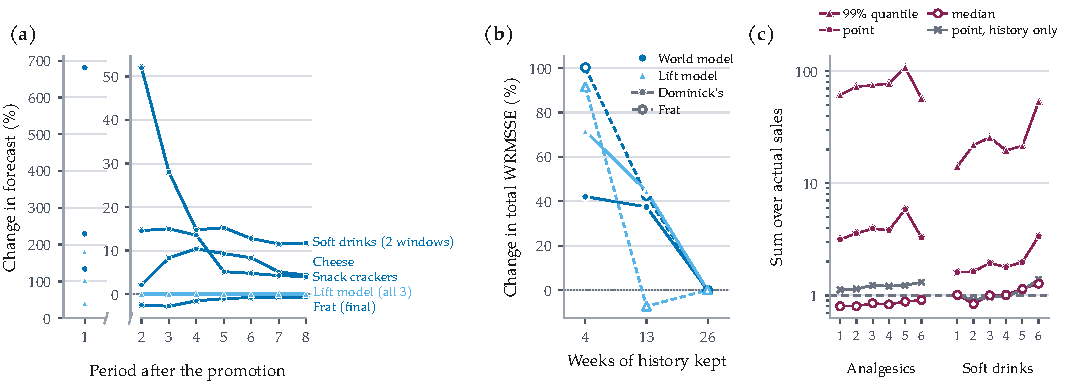
\includegraphics[width=\textwidth]{figs/fig_mechanism.pdf}
\caption{\textbf{The world model carries a promotion forward as further lift and
leans on the most recent weeks; Timestral given the plan puts extreme upper
quantiles on a few series.}
\textbf{(a)} Persistence: the change in the forecast, in percent, at each later
period after one promotion and a 20\% price cut are added in the first period
of the window, for the world model and the lift model (which has no carried
state, so its later change is zero by construction). \textbf{(b)} History
occlusion: the change in total WRMSSE, in percent, when only the last 4 or 13 of
the 26 weeks of history the models read are kept (26: nothing removed). \textbf{(c)} Timestral with the plan on two Dominick's
categories: the sum over all series of its median, its point forecast (the mean
of its quantiles) and its 99\% quantile, over actual sales, per rolling window;
log scale, dashed line at 1. Study B and the mechanism tests use the saved models
with no refitting; (c) from study F.}
\label{fig:mechanism}
\end{figure*}

All three trained models use the plan (Table~\ref{tab:perturbation}). With the
whole plan set to ``nothing planned'' the total error on Dominick's rises by
\rper{dom}{world}{wholeplan}{occlude}{total}\% for the world model,
\rper{dom}{lift}{wholeplan}{occlude}{total}\% for the lift model and
\rper{dom}{lgb}{wholeplan}{occlude}{total}\% for LightGBM, and the forecast in
planned periods changes by \rper{dom}{world}{wholeplan}{occlude}{units}\%,
\rper{dom}{lift}{wholeplan}{occlude}{units}\% and
\rper{dom}{lgb}{wholeplan}{occlude}{units}\%. Price carries more of it than
the promotion flag on Dominick's and Frat. On M5 prices rarely change, and the
plan inputs that matter are event and SNAP days: occluding SNAP days raises the
world model's total error by \rper{mfive}{world}{snap}{occlude}{total}\% and
LightGBM's by \rper{mfive}{lgb}{snap}{occlude}{total}\%, and occluding event days
by \rper{mfive}{world}{event}{occlude}{total}\% against
\rper{mfive}{lgb}{event}{occlude}{total}\%. The world model reads these
calendar inputs more than LightGBM does, which fits its lower error at the M5
total. On Frat the world model gets almost nothing from the
promotion flag once price is given (\rper{frat}{world}{promo}{occlude}{ixs}\%
item by store), while LightGBM and the lift model do.

Three tests on the saved world models show what the carried state does with
the plan. \emph{Timing}: shuffling the plan within each series, with its total
exposure unchanged, raises item-by-store error in cheese by
\rmech{che}{rolling}{world}{bottomchange}\% for the world model and
\rmech{che}{rolling}{lift}{bottomchange}\% for the lift model, and in snack
crackers by \rmech{sna}{rolling}{world}{bottomchange}\% and
\rmech{sna}{rolling}{lift}{bottomchange}\%: both use when the plan falls, and
the carried state adds little to that. \emph{Persistence}
(Figure~\ref{fig:mechanism}a): after a promotion and price cut added in the
first period, the world model's forecast stays higher in later periods, by
\rmech{sna}{rolling}{world}{persisth2}\% one period later in snack crackers and
\rmech{che}{rolling}{world}{persisth3}\% two periods later in cheese, falling
slowly. In categories where shoppers stock up, sales after a promotion dip; the
world model carries the promotion forward as further lift. On Frat the effect
is a small dip (\rmech{frat}{final}{world}{persisth2}\% one period later).
\emph{State}: a ridge read-out from the rolled state predicts sales in the
periods after the window no better than the same read-out from the state before
it ($R^2$ \rmech{che}{rolling}{world}{probeafterr2} against
\rmech{che}{rolling}{world}{probebeforer2} in cheese,
\rmech{mfive}{rolling}{world}{probeafterr2} against
\rmech{mfive}{rolling}{world}{probebeforer2} on M5).

On the weekly data the world model and the lift model read the last 26 weeks of
history, and the most recent weeks matter most (Figure~\ref{fig:mechanism}b):
keeping only the last 13 raises the Dominick's total error by
\rper{dom}{world}{historylast13}{occlude}{total}\% for the world model and
\rper{dom}{lift}{historylast13}{occlude}{total}\% for the lift model, and
keeping only the last 4 by \rper{dom}{world}{historylast4}{occlude}{total}\%
and \rper{dom}{lift}{historylast4}{occlude}{total}\%. On M5, keeping only the
last 28 days raises the world model's total error by
\rper{mfive}{world}{historylast28}{occlude}{total}\% and the lift model's by
\rper{mfive}{lift}{historylast28}{occlude}{total}\%.

\subsection{Pretrained models}
\label{sec:res-pretrained}

\begin{table*}[t]
\centering
\caption{\textbf{Timestral, released two days before this revision, is behind the ensemble on every data set, and
putting it in place of TimesFM helps only at the M5 total.} Mean WRMSSE over the rolling windows (Dominick's: mean
of the six categories). Timestral-28M, zero-shot, the mean of its 21 quantiles as the point forecast; with the plan as
known future inputs (TS+p) and from history alone (TS); TFM+p: TimesFM with the plan. Ens.: the ensemble; Ens.\,T:
Timestral with the plan in place of TimesFM with the plan; Ens.\,4: all four together. Study F, written down before it ran.}
\label{tab:timestral}
\footnotesize
\setlength{\tabcolsep}{3pt}
\begin{tabular}{l*{12}{r}}
\toprule
 & \multicolumn{6}{c}{\textbf{Item by store}} & \multicolumn{6}{c}{\textbf{Total}} \\
\cmidrule(lr){2-7}\cmidrule(lr){8-13}
\textbf{Data} & Ens. & Ens.\,T & Ens.\,4 & TFM+p & TS+p & TS & Ens. & Ens.\,T & Ens.\,4 & TFM+p & TS+p & TS \\
\midrule
Dominick's (six) & \textbf{0.612} & 0.916 & 0.821 & 0.613 & 1.565 & 0.728 & \textbf{0.672} & 3.729 & 2.858 & 0.807 & 10.788 & 2.121 \\
Frat & \textbf{0.549} & 0.623 & 0.595 & 0.578 & 0.864 & 0.792 & 0.337 & 0.501 & 0.407 & \textbf{0.327} & 1.048 & 0.484 \\
M5 & \textbf{0.834} & 0.846 & 0.842 & 0.842 & 0.894 & 0.861 & 0.706 & \textbf{0.609} & 0.699 & 1.035 & 1.025 & 1.014 \\
Favorita & \textbf{0.694} & 0.697 & \textbf{0.694} & 0.712 & 0.731 & 0.771 & 0.303 & \textbf{0.298} & 0.313 & 0.397 & 0.403 & 0.430 \\
\bottomrule
\end{tabular}
\end{table*}


TimesFM with the plan is the most accurate model not trained on the data, and
the plan matters to it: item by store it is ahead of TimesFM from history alone
on every data set where both ran except M5, where they tie
(Table~\ref{tab:rolling}), and most on the weekly
promotion-driven data (soft drinks \rv{sdr}{tfmplan}{ixs} against
\rv{sdr}{tfm}{ixs}). LightGBM is more accurate than it item by store on
\rcount{lgbbeatstfmplanixs} data sets and at the total on
\rcount{lgbbeatstfmplantotal}, and TimesFM with the plan is more accurate than
LightGBM on \rcount{tfmplanbeatslgbixs}.
Chronos-Bolt, from history alone, is behind TimesFM from history alone on every
data set item by store, and its total error in snack crackers is
\rv{sna}{chronos}{total}.

Timestral (study F, Table~\ref{tab:timestral}) is behind the ensemble on every
data set, at both levels. Given the plan it is behind TimesFM given the plan on
every data set except the M5 total, where they tie (\rsf{mfive}{tsplan}{total}
against \rsf{mfive}{tfmplan}{total}). Putting it in place of TimesFM makes the
ensemble less accurate on Dominick's and Frat, level at the Favorita total and
slightly less accurate item by store, and more
accurate only at the M5 total (\rsf{mfive}{enstimestral}{total} against
\rsf{mfive}{ens}{total}); as written down before it ran, the paper's ensemble is
unchanged and that swap is reported as a robustness result. The larger
Timestral-209M, run on Frat to check the model size, is less accurate than the
28M model (\rsf{frat}{tsbig}{ixs} against \rsf{frat}{tsplan}{ixs} item by
store).

On Dominick's Timestral with the plan forecasts several times total sales
(Figure~\ref{fig:mechanism}c). This is not a scale or input error: summed over
all series, its median is \rtail{ana}{tsplan}{median}{lo} to
\rtail{ana}{tsplan}{median}{hi} times actual sales in analgesics, and its
history-only point forecast \rtail{ana}{tsmean}{forecast}{lo} to
\rtail{ana}{tsmean}{forecast}{hi}. Given the plan, its 99\% quantile sums to
\rtail{ana}{tsplan}{q99}{lo} to \rtail{ana}{tsplan}{q99}{hi} times actual sales,
and because the point forecast is the mean of its quantiles, a few series carry
the error: the top 1\% of series by excess hold \rtail{ana}{tsplan}{share}{lo}\%
to \rtail{ana}{tsplan}{share}{hi}\% of it. The same happens more mildly in soft
drinks (99\% quantile \rtail{sdr}{tsplan}{q99}{lo} to
\rtail{sdr}{tsplan}{q99}{hi} times sales) and Frat
(\rtail{frat}{tsplan}{q99}{lo} to \rtail{frat}{tsplan}{q99}{hi}), and not on
the daily data. The forecast rule was not changed after the result. Timestral's
median would sit much closer to sales here, but it is fixed in advance to the
mean, as for Chronos-Bolt, because the median forecasts well below totals for
items that often sell nothing.

\subsection{A data set kept out of development}
\label{sec:res-favorita}

On Favorita, where nothing was tuned and every setting came from the M5
configuration, the ensemble has the lowest error at every level and is alone in
the model confidence set item by store (\rv{fav}{ens}{ixs} against
\rv{fav}{lgb}{ixs} for LightGBM and \rv{fav}{world}{ixs} for the world model);
at the total LightGBM (\rv{fav}{lgb}{total}) and the world model
(\rv{fav}{world}{total}) are in the set with it (\rv{fav}{ens}{total}). The world
model is behind LightGBM at every level, as on most of the other data sets, and
still adds to the ensemble item by store: without it the ensemble's error rises
by \rab{fav}{withoutworldmodel}{ixs}{meandiff}, and with the lift model in its
place by \rab{fav}{liftforworldmodel}{ixs}{meandiff}. The lift model is far
behind at the total (\rv{fav}{lift}{total}). Favorita has no prices, so its
weights are unit weights and its plan is promotions, holidays and paydays.

\subsection{Intervals and ranking}
\label{sec:res-intervals}

\begin{table*}[t]
\centering
\caption{\textbf{Rolling conformal intervals cover close to their level at item by store and somewhat less at the
total, and do not separate the models.} Scaled pinball loss (SPL, lower is better) and the share of actual sales
inside the 80\% and 95\% intervals, mean over the rolling windows after the first. Intervals from each model's own
scaled errors in the earlier windows of the data set, pooled over horizons where a level has fewer than 50 earlier
errors per horizon, ends rounded outwards to whole units except on Favorita (interval check of 16 October).}
\label{tab:intervals}
\footnotesize
\setlength{\tabcolsep}{2.6pt}
\begin{tabular}{l*{18}{r}}
\toprule
 & \multicolumn{9}{c}{\textbf{Item by store}} & \multicolumn{9}{c}{\textbf{Total}} \\
\cmidrule(lr){2-10}\cmidrule(lr){11-19}
 & \multicolumn{3}{c}{Ensemble} & \multicolumn{3}{c}{World} & \multicolumn{3}{c}{LightGBM}
 & \multicolumn{3}{c}{Ensemble} & \multicolumn{3}{c}{World} & \multicolumn{3}{c}{LightGBM} \\
\cmidrule(lr){2-4}\cmidrule(lr){5-7}\cmidrule(lr){8-10}\cmidrule(lr){11-13}\cmidrule(lr){14-16}\cmidrule(lr){17-19}
\textbf{Data} & SPL & 80 & 95 & SPL & 80 & 95 & SPL & 80 & 95 & SPL & 80 & 95 & SPL & 80 & 95 & SPL & 80 & 95 \\
\midrule
Cheese & 0.22 & 0.75 & 0.94 & 0.25 & 0.74 & 0.93 & 0.23 & 0.75 & 0.94 & 0.12 & 0.68 & 0.88 & 0.20 & 0.72 & 0.97 & 0.16 & 0.93 & 0.95 \\
Snack crackers & 0.23 & 0.74 & 0.94 & 0.24 & 0.73 & 0.94 & 0.23 & 0.73 & 0.93 & 0.53 & 0.60 & 0.72 & 0.80 & 0.57 & 0.60 & 0.42 & 0.75 & 0.88 \\
Soft drinks & 0.23 & 0.75 & 0.94 & 0.25 & 0.74 & 0.94 & 0.23 & 0.75 & 0.93 & 0.27 & 0.68 & 0.80 & 0.28 & 0.80 & 0.82 & 0.26 & 0.65 & 0.85 \\
Bottled juice & 0.23 & 0.73 & 0.93 & 0.26 & 0.72 & 0.93 & 0.24 & 0.73 & 0.93 & 0.15 & 0.82 & 0.93 & 0.20 & 0.80 & 0.95 & 0.15 & 0.93 & 0.97 \\
Analgesics & 0.25 & 0.91 & 0.98 & 0.25 & 0.91 & 0.98 & 0.24 & 0.91 & 0.98 & 0.25 & 0.85 & 0.88 & 0.29 & 0.85 & 0.95 & 0.27 & 0.88 & 0.95 \\
Frozen entrees & 0.18 & 0.69 & 0.93 & 0.18 & 0.69 & 0.93 & 0.17 & 0.70 & 0.93 & 0.12 & 0.90 & 0.97 & 0.12 & 0.88 & 1.00 & 0.10 & 0.82 & 0.90 \\
Frat & 0.20 & 0.87 & 0.97 & 0.22 & 0.87 & 0.97 & 0.21 & 0.87 & 0.97 & 0.11 & 0.75 & 0.96 & 0.15 & 0.83 & 0.88 & 0.14 & 0.62 & 0.83 \\
M5 & 0.32 & 0.94 & 0.98 & 0.33 & 0.94 & 0.98 & 0.33 & 0.94 & 0.98 & 0.18 & 0.71 & 0.94 & 0.19 & 0.76 & 0.86 & 0.14 & 0.80 & 0.98 \\
Favorita & 0.24 & 0.79 & 0.95 & 0.25 & 0.79 & 0.95 & 0.24 & 0.79 & 0.95 & 0.07 & 0.83 & 0.98 & 0.10 & 0.70 & 0.93 & 0.07 & 0.86 & 1.00 \\
\bottomrule
\end{tabular}
\end{table*}


The first conformal intervals covered far less than planned at the totals
(95\% intervals holding \rintold{mfive}{ens}{total}{coverage95} of actual sales
at the M5 total for the ensemble and \rintold{frat}{world}{total}{coverage95}
for the world model on Frat), because a level with one node has one earlier
error per horizon per window, so the 2.5\% and 97.5\% quantiles were the
smallest and largest of one to four numbers. With horizons pooled where errors
are few (Table~\ref{tab:intervals}, Figure~\ref{fig:decisions}b) the ensemble's 95\% interval holds
\rint{mfive}{ens}{total}{coverage95} at the M5 total and
\rint{frat}{ens}{total}{coverage95} on Frat. Item by store the 95\% intervals hold
0.93 to 0.98 of sales for all three models, and above 0.95 on M5 and Frat because
rounding a narrow interval outwards to a whole unit widens it; the pinball loss,
unchanged by rounding, is the measure to compare there, and it separates the
three models by at most 0.03 on every data set. Scored on their own
quantiles item by store, TFT's are level with the conformal intervals
(\rint{frat}{tft}{native}{spl} on Frat against \rint{frat}{ens}{ixs}{spl} for
the ensemble) and Chronos-Bolt's are behind them
(\rint{mfive}{chronos}{native}{spl} on M5 against \rint{mfive}{ens}{ixs}{spl}).

The ensemble also ranks item-by-store changes better than any single model
(Figure~\ref{fig:decisions}c). Across item-store series, the Spearman
correlation between forecast and actual change is \rrank{dom}{ens}{ixs}{spearman}
on Dominick's, \rrank{fav}{ens}{ixs}{spearman} on Favorita,
\rrank{frat}{ens}{ixs}{spearman} on Frat and \rrank{mfive}{ens}{ixs}{spearman}
on M5, above every single model in the check on each; of the tenth of
series it forecasts to grow most, \rrank{dom}{ens}{ixs}{topdecilehit},
\rrank{fav}{ens}{ixs}{topdecilehit}, \rrank{frat}{ens}{ixs}{topdecilehit} and
\rrank{mfive}{ens}{ixs}{topdecilehit} are in the actual top tenth, against
0.10 by chance. Over promoted periods LightGBM and the ensemble rank promotions best
(\rrank{dom}{lgb}{ixs}{promospearman} and \rrank{dom}{ens}{ixs}{promospearman}
on Dominick's). The ensemble's total forecast is within 6\% of actual sales on
every data source (\rrank{mfive}{ens}{ixs}{totalratio} on M5 is the furthest).

\subsection{Decisions and reconciliation}
\label{sec:res-decisions}
\label{sec:res-recon}

\begin{table*}[t]
\centering
\caption{\textbf{For category plans the world model alone has the lowest cost on \rcount{decworldcat} of eight data sets;
for store orders the ensemble or LightGBM has the lowest cost on every one.} Cost relative to seasonal naive (below 1 is better), mean over the rolling
windows. Category plan: absolute error of each category-by-store total over the window, weighted by dollar sales.
Store orders: order the model's 80\% interval quantile for each item, store and period; each unit over costs 1 and each
unit short costs 4. Simulations under stated costs, not business results. Bold: the lowest in the group.}
\label{tab:decisions}
\footnotesize
\setlength{\tabcolsep}{3.6pt}
\begin{tabular}{l*{10}{r}}
\toprule
 & \multicolumn{5}{c}{\textbf{Category plan}} & \multicolumn{5}{c}{\textbf{Store orders (ratio 0.8)}} \\
\cmidrule(lr){2-6}\cmidrule(lr){7-11}
\textbf{Data} & Ens. & World & Lift & LGB & TFM+p & Ens. & World & Lift & LGB & TFM+p \\
\midrule
Cheese & 0.26 & \textbf{0.12} & 0.16 & 0.30 & 0.36 & 0.52 & 0.55 & 0.57 & \textbf{0.52} & 0.62 \\
Snack crackers & 0.46 & \textbf{0.43} & 0.50 & 0.46 & 0.48 & 0.72 & 0.77 & 0.77 & \textbf{0.71} & 0.76 \\
Soft drinks & 0.19 & \textbf{0.08} & 0.14 & 0.17 & 0.33 & 0.59 & 0.61 & 0.64 & \textbf{0.57} & 0.69 \\
Bottled juice & 0.23 & \textbf{0.12} & 0.18 & 0.28 & 0.29 & \textbf{0.48} & 0.49 & 0.51 & 0.49 & 0.54 \\
Analgesics & 0.41 & 0.43 & 0.39 & \textbf{0.38} & 0.42 & 0.68 & 0.70 & 0.71 & \textbf{0.68} & 0.71 \\
Frozen entrees & 0.17 & \textbf{0.07} & 0.19 & 0.17 & 0.27 & 0.51 & 0.52 & 0.60 & \textbf{0.51} & 0.63 \\
Frat & \textbf{0.50} & 0.57 & 0.56 & 0.51 & 0.52 & \textbf{0.50} & 0.53 & 0.52 & 0.52 & 0.56 \\
M5 & 0.64 & \textbf{0.63} & 1.32 & 0.65 & 0.84 & \textbf{0.82} & 0.83 & 0.88 & 0.85 & 0.83 \\
\bottomrule
\end{tabular}
\end{table*}


\begin{figure*}[t]
\centering
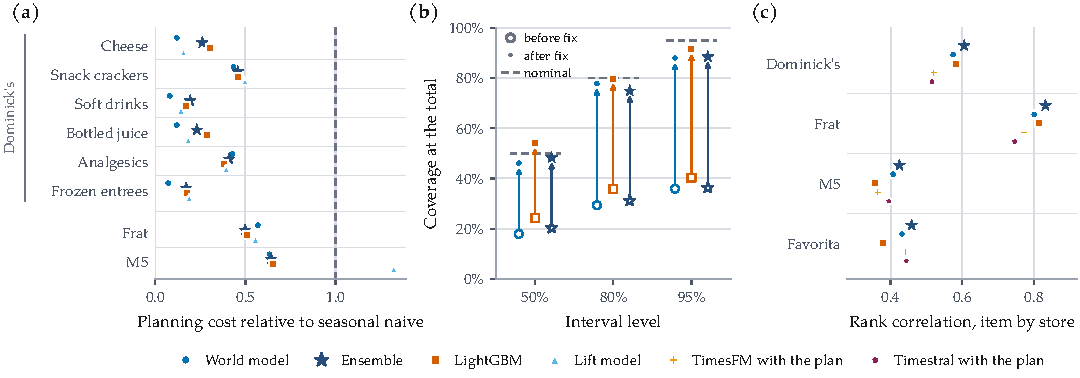
\includegraphics[width=\textwidth]{figs/fig_decisions.pdf}
\caption{\textbf{The world model has the lowest category-plan cost on most data
sets, pooling fixed the interval coverage at the totals, and the ensemble ranks
changes best.} \textbf{(a)} Category-plan cost relative to seasonal naive
(dashed line at 1), mean over the rolling windows. \textbf{(b)} Share of actual
sales inside the 50\%, 80\% and 95\% intervals at the chain total, mean over
the eight data sets scored both before the interval fix (open) and after it
(filled); dashes: the nominal level. \textbf{(c)} Spearman correlation across
item-store series between forecast and actual change, mean over the rolling
windows (Dominick's: over its six categories).}
\label{fig:decisions}
\end{figure*}

The two decisions point to different models (Table~\ref{tab:decisions},
Figure~\ref{fig:decisions}a). For the
category plan, the world model alone has the lowest cost on
\rcount{decworldcat} of eight data sets (\rcount{decworldcatlist}), at
\rdec{fre}{categoryplanning}{world} of seasonal naive's cost in frozen entrees
against \rdec{fre}{categoryplanning}{ens} for the ensemble and
\rdec{fre}{categoryplanning}{lgb} for LightGBM. Its category-by-store totals
over the window are close even where its item forecasts are behind LightGBM's.
For store orders
at a critical ratio of 0.8, LightGBM has the lowest cost on
\rcount{declgborder} (\rcount{declgborderlist}) and the ensemble on
\rcount{decensorder} (\rcount{decensorderlist}); the world model on none.

\begin{table}[t]
\centering
\caption{\textbf{Reconciled ETS forecasts are far behind the trained models; reconciling a trained model's item
forecasts with ETS above them helps on Frat and hurts on M5.} Mean WRMSSE over the rolling windows. MinT with a shrunk
covariance was computed only where the hierarchy has at most 6,000 nodes; on Frat it gave a total WRMSSE of
\rrec{frat}{etsmintshrink}{total}, a numerical failure not investigated further.}
\label{tab:reconcile}
\footnotesize
\setlength{\tabcolsep}{3pt}
\begin{tabular}{p{0.42\columnwidth}rrrr}
\toprule
 & \multicolumn{2}{c}{\textbf{Frat}} & \multicolumn{2}{c}{\textbf{M5}} \\
\cmidrule(lr){2-3}\cmidrule(lr){4-5}
\textbf{Method} & I$\times$S & Total & I$\times$S & Total \\
\midrule
ETS, bottom-up & 0.909 & 0.566 & 0.898 & 1.271 \\
ETS, top-down & 0.806 & 0.487 & 0.917 & 0.902 \\
ETS, OLS & 0.953 & 0.520 & 0.888 & 0.902 \\
ETS, WLS structural & 0.912 & 0.538 & 0.885 & 0.908 \\
ETS, WLS variance & 0.903 & 0.511 & 0.884 & 0.946 \\
ETS, MinT shrink & 0.926 & 247.170 & -- & -- \\
LightGBM + ETS, WLS variance & 0.581 & 0.304 & 0.855 & 0.763 \\
World model + ETS, WLS variance & 0.602 & 0.343 & 0.849 & 0.754 \\
\midrule
LightGBM, unreconciled & 0.570 & 0.360 & 0.861 & 0.693 \\
World model, unreconciled & 0.595 & 0.457 & 0.851 & 0.609 \\
Ensemble, unreconciled & 0.549 & 0.337 & 0.834 & 0.706 \\
\bottomrule
\end{tabular}
\end{table}


Reconciliation does not replace a model trained on the plan
(Table~\ref{tab:reconcile}). The best reconciled ETS forecast on Frat is
top-down, at \rrec{frat}{etstopdown}{ixs} item by store against
\rv{frat}{lgb}{ixs} for LightGBM. Combining a trained model's item forecasts
with ETS above them by weighted least squares lowers the Frat total error
(LightGBM \rrec{frat}{lightgbmwithetswlsvar}{total} against
\rv{frat}{lgb}{total} unreconciled; world model
\rrec{frat}{worldmodelwithetswlsvar}{total} against \rv{frat}{world}{total})
and raises the M5 total error (world model
\rrec{mfive}{worldmodelwithetswlsvar}{total} against
\rv{mfive}{world}{total}). MinT with a shrunk covariance gave a total WRMSSE of
\rrec{frat}{etsmintshrink}{total} on Frat, a numerical failure we did not
investigate further.

\subsection{The final windows of the first version}
\label{sec:res-final}

\begin{table*}[t]
\centering
\caption{\textbf{On M5 the best model depends on the level scored and on the month.} WRMSSE on the four 28-day
windows (lower is better), mean over seeds; seeds per window in the second column. All: the 12 levels together;
Total: the chain total; I$\times$S: item by store. The lowest value in each column is in bold. TimesFM with the
plan has no recorded total. The lift model's April mean includes one failed seed (2.603 overall;
\S\ref{sec:failures}).}
\label{tab:m5}
\footnotesize
\setlength{\tabcolsep}{3.6pt}
\begin{tabular}{lc*{12}{r}}
\toprule
 & & \multicolumn{3}{c}{\textbf{29 Feb to 27 Mar}} & \multicolumn{3}{c}{\textbf{28 Mar to 24 Apr}} & \multicolumn{3}{c}{\textbf{25 Apr to 22 May (practice)}} & \multicolumn{3}{c}{\textbf{23 May to 19 Jun (test)}} \\
\cmidrule(lr){3-5}\cmidrule(lr){6-8}\cmidrule(lr){9-11}\cmidrule(lr){12-14}
\textbf{Model} & \textbf{Seeds} & All & Total & I$\times$S & All & Total & I$\times$S & All & Total & I$\times$S & All & Total & I$\times$S \\
\midrule
World model & 3/3/3/3 & \textbf{0.642} & \textbf{0.398} & 0.851 & \textbf{0.555} & \textbf{0.283} & 0.833 & 0.656 & 0.535 & 0.834 & 0.638 & 0.379 & 0.897 \\
Lift model & 3/3/3/3 & 0.664 & 0.427 & 0.846 & 1.246 & 0.964 & 0.834 & 0.713 & 0.623 & 0.832 & 0.663 & 0.368 & 0.896 \\
LightGBM & 3/3/1/3 & 0.709 & 0.578 & 0.873 & 0.557 & 0.351 & 0.846 & 0.715 & 0.659 & 0.847 & \textbf{0.547} & \textbf{0.247} & 0.905 \\
Graph model & 3/3/3/3 & 0.778 & 0.621 & 0.878 & 0.644 & 0.493 & 0.845 & \textbf{0.641} & \textbf{0.455} & 0.851 & 0.673 & 0.412 & 0.909 \\
TimesFM & 1/1/1/1 & 0.854 & 0.830 & \textbf{0.836} & 0.819 & 0.786 & \textbf{0.828} & 0.896 & 0.930 & \textbf{0.828} & 0.729 & 0.558 & 0.885 \\
TimesFM with the plan & 1/1/1/1 & 0.858 & -- & 0.837 & 0.772 & -- & 0.829 & 0.929 & -- & 0.830 & 0.719 & -- & \textbf{0.883} \\
Seasonal naive & 1/1/1/1 & 0.889 & 0.658 & 1.121 & 0.923 & 0.668 & 1.126 & 0.870 & 0.751 & 1.100 & 0.847 & 0.560 & 1.176 \\
\bottomrule
\end{tabular}
\end{table*}

\begin{table*}[t]
\centering
\caption{\textbf{On the promotion-driven weekly data, models that see the plan lead, and which one leads
changes by category.} WRMSSE on the final 8 weeks (lower is better). World model, lift model and LightGBM:
mean of three seeds, settings fixed on the development windows. TimesFM and TimesFM with the plan: one run each,
added after the final tests. The lift model was run on Frat only. The lowest value in each row and group is in bold.}
\label{tab:finals}
\footnotesize
\setlength{\tabcolsep}{4pt}
\begin{tabular}{l*{10}{r}}
\toprule
 & \multicolumn{5}{c}{\textbf{All levels}} & \multicolumn{5}{c}{\textbf{Item by store}} \\
\cmidrule(lr){2-6}\cmidrule(lr){7-11}
\textbf{Data} & World & Lift & LightGBM & TimesFM & TimesFM+plan & World & Lift & LightGBM & TimesFM & TimesFM+plan \\
\midrule
Frat & 0.681 & 0.714 & \textbf{0.549} & 0.965 & 0.686 & 0.665 & 0.677 & \textbf{0.608} & 0.827 & 0.641 \\
\addlinespace[2pt]
\multicolumn{11}{l}{\itshape Dominick's} \\
Cheese & 0.897 & -- & 0.708 & 0.829 & \textbf{0.545} & 0.715 & -- & 0.702 & 0.792 & \textbf{0.699} \\
Snack crackers & 0.448 & -- & \textbf{0.412} & 0.468 & 0.475 & 0.608 & -- & \textbf{0.596} & 0.640 & 0.614 \\
Soft drinks & \textbf{0.830} & -- & 0.989 & 1.070 & 0.974 & 0.734 & -- & \textbf{0.652} & 0.895 & 0.780 \\
Bottled juice & 0.987 & -- & 0.994 & \textbf{0.940} & 0.990 & 0.816 & -- & \textbf{0.750} & 0.782 & 0.754 \\
Analgesics & \textbf{0.867} & -- & 0.978 & 1.009 & 0.889 & \textbf{0.713} & -- & 0.714 & 0.790 & 0.742 \\
Frozen entrees & 0.485 & -- & \textbf{0.478} & 0.563 & 0.566 & 0.557 & -- & \textbf{0.529} & 0.682 & 0.599 \\
\bottomrule
\end{tabular}
\end{table*}

\begin{table*}[t]
\centering
\caption{\textbf{On the single final windows the ensemble is lowest or within \rcount{finalsgap} of the lowest item by
store on every data set, and the order at the total changes from data set to data set.} WRMSSE on the final
window of each data set (lower is better; on M5 the official test month). One fit (seed~1) per trained model, so the world
model and LightGBM differ slightly from the three-seed means of Tables~\ref{tab:m5} and~\ref{tab:finals}. Bold:
lowest in the group.}
\label{tab:finalsnew}
\footnotesize
\setlength{\tabcolsep}{3pt}
\begin{tabular}{l*{14}{r}}
\toprule
 & \multicolumn{7}{c}{\textbf{Item by store}} & \multicolumn{7}{c}{\textbf{Total}} \\
\cmidrule(lr){2-8}\cmidrule(lr){9-15}
\textbf{Data} & Ens. & World & Lift & LGB & TFM+p & Chr. & TFT & Ens. & World & Lift & LGB & TFM+p & Chr. & TFT \\
\midrule
Cheese & \textbf{0.675} & 0.712 & 0.756 & 0.699 & 0.704 & 0.807 & 0.731 & 0.753 & 1.064 & 0.997 & 0.768 & 0.531 & 1.009 & \textbf{0.522} \\
Snack crackers & \textbf{0.585} & 0.610 & 0.620 & 0.603 & 0.624 & 0.661 & 0.621 & 0.334 & 0.484 & 0.302 & 0.317 & 0.362 & 0.327 & \textbf{0.219} \\
Soft drinks & 0.674 & 0.709 & 0.772 & \textbf{0.655} & 0.780 & 0.912 & 0.849 & 1.065 & \textbf{0.891} & 0.920 & 1.238 & 1.140 & 1.385 & 1.228 \\
Bottled juice & 0.760 & 0.849 & 0.807 & 0.756 & \textbf{0.754} & 0.785 & 0.775 & 1.111 & 1.019 & 1.190 & 1.171 & 1.172 & 1.046 & \textbf{1.015} \\
Analgesics & \textbf{0.710} & 0.712 & 0.714 & 0.716 & 0.742 & 0.802 & 0.770 & 1.236 & 1.186 & 1.280 & 1.407 & 1.149 & 1.454 & \textbf{0.878} \\
Frozen entrees & 0.543 & 0.574 & 0.563 & \textbf{0.530} & 0.599 & 0.692 & 0.557 & 0.454 & 0.423 & \textbf{0.404} & 0.438 & 0.537 & 0.536 & 0.414 \\
Frat & \textbf{0.604} & 0.671 & 0.662 & 0.613 & 0.644 & 0.856 & 0.702 & 0.586 & 0.681 & 0.698 & \textbf{0.523} & 0.677 & 1.222 & 0.818 \\
M5 & \textbf{0.881} & 0.896 & 0.896 & 0.905 & 0.883 & 0.899 & -- & \textbf{0.240} & 0.363 & 0.424 & 0.245 & 0.556 & 1.007 & -- \\
\bottomrule
\end{tabular}
\end{table*}


The first version scored each data set once, on its final window, and its
findings stand: on M5 the most accurate model depended on the level and the
month (Table~\ref{tab:m5}), and on Dominick's and Frat on the category
(Table~\ref{tab:finals}). On M5, TimesFM given only history was the most
accurate single model item by store in all four months (\mTfmTestIxs{} on the
test month, against \mWorldTestIxs{} for the world model and \mLgbTestIxs{} for
LightGBM), while the plan-aware models were far more accurate at the totals. The
official test month was the only one of four in which LightGBM was the most
accurate over all levels (\mLgbTestOverall{} against \mWorldTestOverall), so a
comparison on that month alone would have ranked it first. Run on the final
windows (Table~\ref{tab:finalsnew}), the ensemble is lowest or within
\rcount{finalsgap} of the lowest item by store on every data set, which agrees
with the rolling windows.

\begin{figure*}[t]
\centering
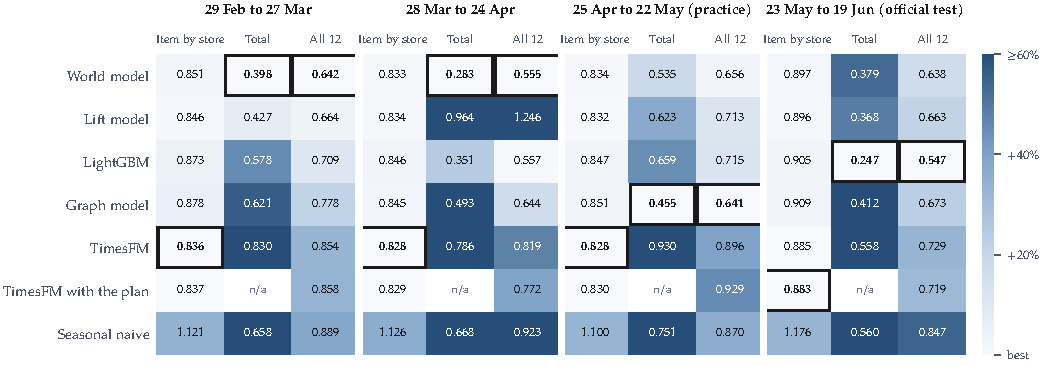
\includegraphics[width=\textwidth]{figs/fig_m5_heat.pdf}
\caption{\textbf{On the M5 final windows, TimesFM from history alone had the
lowest item-by-store error of the single models in every month; at the total and
over all levels the plan-aware models did, and which one changed by month.}
WRMSSE of every single model, four windows, three levels; cell shade: how far
above the lowest value in its column (white: the lowest, outlined). Trained
models: mean of three seeds. The lift model's April mean includes one failed
seed (\S\ref{sec:dropped}).}
\label{fig:m5heat}
\end{figure*}

\paragraph{How much the plan matters}
On M5, where prices rarely change, giving TimesFM the plan changed its
item-by-store error by at most 0.002 in any month. On Dominick's, where promoted
weeks carry \promoShareLo\% to \promoShareHi\% of a category's units, TimesFM
without the plan forecast \promoTfmLo\% to \promoTfmHi\% of promoted-week sales
and with it \promoTfmPlanLo\% to \promoTfmPlanHi\%
(Figure~\ref{fig:planarrows}a). The trained plan-aware models also fell short in
promoted weeks: the world model forecast \promoWorldLo\% to \promoWorldHi\% of
promoted-week sales and LightGBM \promoLgbLo\% to \promoLgbHi\%.

\begin{figure*}[t]
\centering
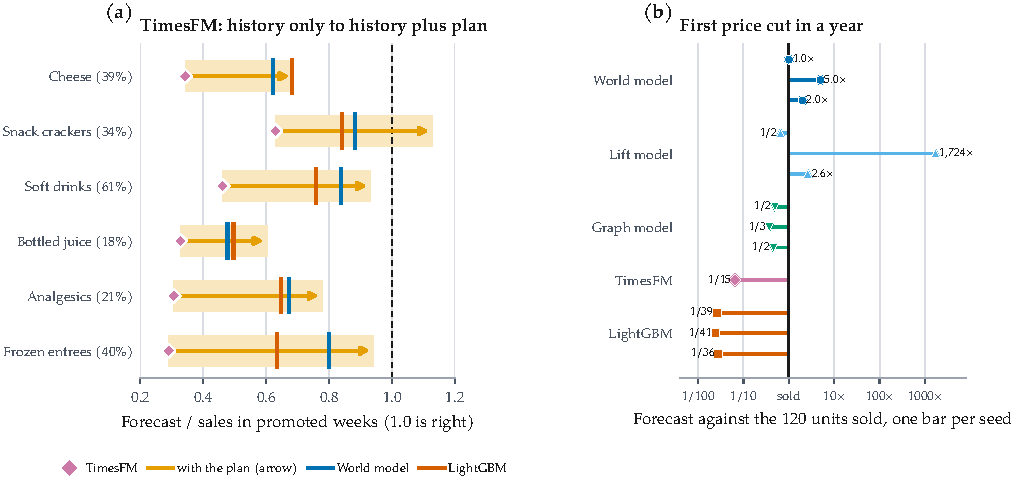
\includegraphics[width=\textwidth]{figs/fig_plan_arrows.pdf}
\caption{\textbf{Given the plan, TimesFM closes most of its promoted-week
shortfall; for a price cut history has not shown, plan-aware models respond and
history-only models do not.} \textbf{(a)} Forecast against sales in the promoted
weeks of the final 8 weeks, by Dominick's category (promoted weeks' share of the
category's units in brackets): TimesFM from history alone (diamond) to TimesFM
with the plan (arrow head), with the world model and LightGBM (ticks). \textbf{(b)}
HOUSEHOLD\_1\_146 in the four M5 stores where it had its first price cut in a year
(5.98 to 4.50 for one week) inside the April window: each seed's forecast over
the 28 days against the \cutSold{} units sold, log scale.}
\label{fig:planarrows}
\end{figure*}

\paragraph{First-time price cuts}
In the April M5 window, HOUSEHOLD\_1\_146 had sold almost nothing for a year at
5.98, then sold \cutSold{} units in four stores over a window that held a
one-week cut to 4.50 (Figure~\ref{fig:planarrows}b). Models working from history
forecast almost nothing: LightGBM \cutLgb{} units across seeds, TimesFM
\cutTfm. The world model, which reads the cut through its plan, forecast
\cutWorld; the graph model \cutGraph; the lift model \cutLift. How large the
response should be is not fixed by the data: the world-model seeds differ by a
factor of five, and one lift-model seed forecast over 200,000 units.

% =====================================================================
\section{What was tried and dropped}
\label{sec:dropped}

We report the failures at the same length as the results.
Table~\ref{tab:dropped} lists what this revision tried and did not keep, and
Table~\ref{tab:ledger} what the first version did.

\begin{table*}[t]
\centering
\caption{\textbf{What the revision tried and did not keep.} Each was written
down with its pass rule before it ran. dev.: the development windows of the six
Dominick's categories. After promotion: forecast over actual in the two periods
after a promotion.}
\label{tab:dropped}
\footnotesize
\renewcommand{\arraystretch}{1.15}
\begin{tabular}{p{0.26\textwidth}p{0.21\textwidth}p{0.45\textwidth}}
\toprule
\textbf{Change or model} & \textbf{Where tested} & \textbf{Result} \\
\midrule
Stock term on the world model (study C) & Dominick's dev., seed 1 & Overall worse than the world model in three of six categories \\
Plan of the two periods before, on the lift model (study C) & Dominick's dev., seed 1 & Overall worse than the world model in three of six \\
Stock term on the lift model (study C) & Dominick's dev., then rolling & Passed on development (after promotion \rpan{dev}{sdr}{liftstock}{mean}{afterpromofa} soft drinks, \rpan{dev}{sna}{liftstock}{mean}{afterpromofa} snack crackers); on the rolling windows \rpan{rol}{sdr}{liftstock}{roll}{afterpromofa} and \rpan{rol}{sna}{liftstock}{roll}{afterpromofa}, against \rpan{rol}{sdr}{worldmodel}{roll}{afterpromofa} and \rpan{rol}{sna}{worldmodel}{roll}{afterpromofa} for the world model \\
Weight 3 on periods after a promotion (study E) & Dominick's dev., seed 1 & Error after promotion lower in all six (soft drinks \raft{sdr}{worldmodel}{afterpromoerr} to \raft{sdr}{afterpromow2}{afterpromoerr}); overall worse in four (snack crackers \raft{sna}{worldmodel}{overall} to \raft{sna}{afterpromow2}{overall}) \\
Weight 6 on periods after a promotion (study E) & Dominick's dev., seed 1 & Overall worse in four; snack crackers after promotion \raft{sna}{afterpromow5}{afterpromofa} \\
Fitted ensemble weights (study A) & All nine, rolling & Better than equal weights in \rcount{fittedwins} of \rcount{fittedn} comparisons, worse in \rcount{fittedlosses} \\
Timestral in place of TimesFM (study F) & All four sources, rolling & Worse on Dominick's and Frat; better at the M5 total only \\
Timestral-209M (study F) & Frat, rolling & Less accurate than 28M; too slow for the other data sets \\
MinT, shrunk covariance & Frat, rolling & Total WRMSSE \rrec{frat}{etsmintshrink}{total}; not investigated \\
\bottomrule
\end{tabular}
\end{table*}

\begin{table*}[t]
\centering
\caption{\textbf{Every change and comparison model that did not become a default.} Overall WRMSSE unless
stated; ``against'' gives the default it was compared with on the same window. dev.: development windows before
the final 8 weeks. Practice: the M5 window 25 April to 22 May 2016. Each row is a section of
\texttt{results/README.md} with its run folders.}
\label{tab:ledger}
\footnotesize
\begin{tabular}{p{0.30\textwidth}p{0.28\textwidth}p{0.34\textwidth}}
\toprule
\textbf{Change or model} & \textbf{Where tested} & \textbf{Result} \\
\midrule
Twice the training steps & Dominick's (6) and Frat, dev., 3 seeds & Better in 2, worse in 3, level or mixed in 2 \\
Weekday as seven inputs & M5 practice, seed 1 & 0.653 against 0.646 \\
Event kinds (with weekday) & M5 practice, seed 1 & 0.646 against 0.646 \\
60,000 training steps & M5 practice, seed 1 & 0.642 against 0.646; gain below seed range 0.029 \\
Item level against past-year level & M5 practice, seed 1 & 0.680 against 0.646 \\
Totals term in the loss & Dominick's analgesics, dev. & 0.819 against 0.683; total 8\% under \\
Negative binomial likelihood & Frat, analgesics, dev. & Level \\
Plan split, latent check, near-week weighting & Frat, dev., 5 seeds & 0.417 to 0.427 against 0.408 \\
Own forecast fed into the roll-forward & Dominick's (6), dev. & Worse overall in 4 of 6 \\
Item role labels & Dominick's (6), dev. & No effect on LightGBM; snack crackers 2.422 for the world model \\
Averaging three fits & M5 practice, seed 1 & 0.665 against 0.656 (kept on Dominick's) \\
Graph model over product attributes & M5, four windows, 3 seeds & Level with LightGBM item by store \\
TimesFM, median output & M5, four windows & Overall 1.71 to 1.88; totals 27\% to 31\% under \\
Lift model (no roll-forward) & M5, four windows, 3 seeds & One seed failed in April (2.603) \\
\bottomrule
\end{tabular}
\end{table*}


\paragraph{The forecast after a promotion}
The persistence test showed the world model carrying a promotion forward as
further lift where shoppers stock up. Studies C and E tried to give the dip a
route. A stock term, one number per item that builds with sales above the
item's level, decays by a learnt share and lowers later sales by a learnt amount
that cannot be negative, made the world model worse overall in three of six
categories on the development windows. On the lift model it passed the
development rule, but on the rolling windows it did not fix the after-promotion
forecast (soft drinks \rpan{rol}{sdr}{liftstock}{roll}{afterpromofa} with it,
\rpan{rol}{sdr}{lift}{roll}{afterpromofa} for the plain lift model,
\rpan{rol}{sdr}{worldmodel}{roll}{afterpromofa} for the world model). A loss
weight on the periods after a promotion lowered the error there in all six
categories and made the overall score worse in four. None became a default. The
reason given for study C also needed a correction: the 1.32 and 1.33
after-promotion ratios that prompted it came from an earlier world-model
version; the final world model was at 1.00 and 1.04 on those windows.

\paragraph{A seed that never reached single fits, and noise as large as the
effects}
Stage 2 of study C repeated each configuration with seeds 2 and 3 and got
identical scores in all twelve runs. Single-fit configurations whose settings
named no seed trained with seed 0 for every run seed; the seed now reaches the
model, and the results already recorded are those of seed 0 (each manifest
records its commit). The repeat also showed that two runs of the same
configuration on different Colab machines differ by as much as the variants
being tested: the world model's overall score in snack crackers was
\rpan{dev}{sna}{worldmodel}{a}{overall} on one machine and
\rpan{dev}{sna}{worldmodel}{b}{overall} on another. Study E therefore reran the
world model in the same job as the variants it was compared with. The rolling
windows, being one fit per model, carry this noise; the paired tests over
windows absorb part of it, not all.

\paragraph{A lift-model seed that broke on five series}
In the April M5 final window, lift-model seed 2 scored \mLiftAprSeedBOverall{}
over all levels against \mLiftAprSeedAOverall{} and \mLiftAprSeedCOverall{} for
seeds 1 and 3, and forecast \liftSeedTwoForecast{} units against
\liftSeedTwoSold{} sold. Five item-store series hold all of the excess, each with
its first price cut in a year inside the window; the seed read the cuts as lifts
up to the model's bound. Item by store, weighted by dollar sales, the failure is
invisible (\mLiftAprIxs); at the totals it dominates. The world model did not
fail on these series in any seed.

\begin{figure*}[t]
\centering
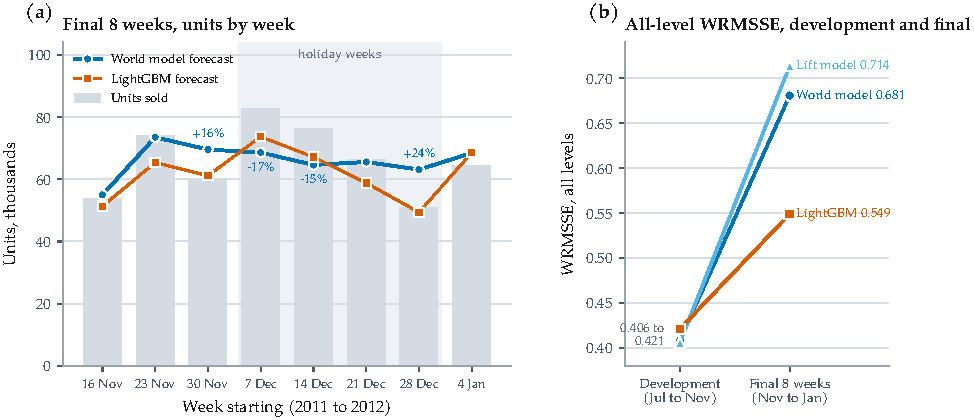
\includegraphics[width=\textwidth]{figs/fig_frat_story.pdf}
\caption{\textbf{On the Frat final window the world model got the 8-week total
right and missed the holiday shape, which the development windows did not
contain.} \textbf{(a)} Units sold each week of the final window over all
item-stores (bars), and the weekly forecasts of the world model and LightGBM,
three seeds averaged; labels: the world model's largest weekly misses.
\textbf{(b)} All-level WRMSSE on the development windows and on the final 8 weeks.}
\label{fig:fratstory}
\end{figure*}

\paragraph{Frat holiday weeks}
On the Frat development windows the world model, lift model and LightGBM were
level (0.406 to 0.421). On the final 8 weeks the world model fell to
\fWorldFratOverall{} against \fLgbFratOverall{} for LightGBM. The final weeks
are the holiday period, which the development windows did not contain
(Figure~\ref{fig:fratstory}); the world model's 8-week total is right (forecast
against sales \fWorldFratFa) but it is 15\% to 17\% under in the two December
peak weeks. LightGBM, with week-of-year and month inputs and the previous
holiday season in its training data, follows that shape more closely.

\paragraph{TimesFM's default output}
TimesFM's default point forecast is the median. For an item that sells nothing
on most days the median is near zero while the mean is not, so the median
forecast is 27\% to 31\% below M5 totals in every month. The mean output, used
throughout, does not have the problem.

% =====================================================================
\section{Discussion}
\label{sec:discussion}

A retailer that knows its plan should forecast items with an equal-weight
average of a plan-aware world model, a tree model and a pretrained model given
the plan, and should check the category totals against the world model alone
(Table~\ref{tab:advice}).

\begin{table*}[t]
\centering
\caption{\textbf{Each decision has its own level, and the results point to a
forecast for each.}}
\label{tab:advice}
\footnotesize
\renewcommand{\arraystretch}{1.2}
\begin{tabular}{p{0.23\textwidth}p{0.18\textwidth}p{0.51\textwidth}}
\toprule
\textbf{Decision} & \textbf{Level} & \textbf{What the results say} \\
\midrule
Store orders and inventory & Item by store, day or week & The ensemble or LightGBM: lowest order cost on every data set; the ensemble lowest item-by-store error on \rcount{enslowestixs} of nine \\
Promotion, price change, supplier funding & Item by week, under a planned change & A model that reads the plan; history alone forecasts \promoTfmLo\% to \promoTfmHi\% of promoted-week sales. Check forecasts after a promotion in categories where shoppers stock up: the world model carries the lift forward \\
Category sales, units and margin plans & Category or chain, week or month & The world model alone: lowest category-plan cost on \rcount{decworldcat} of eight; the ensemble at the total is in the confidence set everywhere \\
Choosing a model & Any & Score several windows with paired tests; one test month reversed the ranking on M5, and runs on different machines differed by as much as the changes tested \\
Adopting a new pretrained model & Any & Check its totals and its upper quantiles before use; Timestral's tails made its mean forecast several times sales on weekly data \\
\bottomrule
\end{tabular}
\end{table*}

\paragraph{Why an equal-weight ensemble}
The three members fail in different places. LightGBM is the most accurate single
model item by store on most data sets and the member the ensemble can least do
without. TimesFM with the plan brings a pretrained view of each series' history.
The world model has the lowest category-plan cost on \rcount{decworldcat} of
eight data sets, and the ensemble without it is less accurate item by store on
\rcount{withoutworldmodelixsens}. An average of three models whose errors
differ is more accurate item by store than any of them on
\rcount{enslowestixs} of nine data sets, and equal weights are as good as weights fitted on a few earlier
windows, as the forecast combination literature leads one to
expect~\cite{smithwallis2009,wang2023}.

\paragraph{What the carried state adds}
Against the lift model, which differs only in the carried state, the world model
is level on its own in most data sets, adds to the ensemble beyond the lift
model on \rcount{liftforworldmodelixsens} data sets item by store and
\rcount{liftforworldmodeltotalens} at the total, and has a lower category-plan
cost than the lift model on \rcount{worldbeatsliftcat} of eight. The carried state holds the plan (Figure~\ref{fig:readback}), but the
rolled state does not predict sales beyond the window better than the state
before it, and it carries a promotion forward as more lift rather than a dip.
On these data the case for the carried state is what it adds to an ensemble and
to category totals, not item accuracy on its own.

\paragraph{Two cautions}
A plan-driven forecast responds to plans unlike history with a size the data do
not fix: one lift-model seed and Timestral's upper quantiles both produced
forecasts many times any sale. And a forecast that is accurate item by store
can be several percent off the category total, which is the number a merchant
plans against.

% =====================================================================
\section{Limitations and threats to validity}
\label{sec:limitations}

\paragraph{Windows and seeds}
Trained models are one fit each in the rolling windows, and runs of one
configuration on different machines differed by as much as some differences
tested (\S\ref{sec:dropped}). Four to six windows per data set give wide
intervals across windows, so ``level'' often means ``not separated''. Single-fit
runs before 16 October trained with seed 0 whatever seed was named.

\paragraph{Studies added after the main results}
Studies A to F were added after the rolling results were read. Each was written
down before it ran, but which studies to run was chosen knowing that the
ensemble came first. Timestral was run at 28M parameters, not 209M, because the
larger model was too slow, a change made before any Timestral result.

\paragraph{Comparison models}
TFT was not run on M5 or Favorita, and Chronos-Bolt and TimesFM from history
alone not on Favorita. TimesFM with the plan fits its linear plan model within
groups of 2,048 series. Pretrained models are used as published with their point
forecast fixed in advance (the mean), which for Timestral was the wrong choice on
weekly data.

\paragraph{What lift means}
Merchants promote in weeks they expect to sell well, so part of a measured lift
is good timing. The lift is what the forecast attributes to the plan, not what
the plan caused. Our companion audit~\cite{paper2} measures the gap in generated
store data where the true lifts are known: the world model's and LightGBM's
lifts were a third too large while every check against the model passed. Plan
responses in this paper, including the perturbation tests, are forecasts, not
causal estimates.

\paragraph{What the data do not record}
None of the data sets records stock, so a sell-out looks like low demand; or
shelf space. Favorita records no prices. The data were collected between 1989
and 2017 and their plan inputs differ, so the results compare models within each
data set. The decision costs are simulations under stated costs.

% =====================================================================
\section{Conclusion}
\label{sec:conclusion}

An equal-weight ensemble of a world model, LightGBM and TimesFM given the plan
is the most accurate item-by-store forecast on rolling windows of four public
retail data sets, including one kept out of development, and it is never less
accurate than LightGBM or the world model by a paired test. The world model
adds to it on some data sets, and its carried state on fewer; on its own it is
behind LightGBM item by store and gets category totals right. Every trained model
uses the plan, the world model carries promotions forward as further lift, and a
pretrained model released this month needs its tails checked before use.
Retail forecasts should be chosen by the decision they feed, at that decision's
level, over several windows with paired tests, with the losing models stated.

\section{Reproducibility and compute}
\label{sec:repro}

\paragraph{Records}
All code, configuration files and tests are in the repository. A run refuses to
start on uncommitted code and writes a manifest holding the code commit, the
full configuration and its checksum, the seed, checksums of every data file
read, package versions, the machine and run times. The manifest and scores of
the \nPromotedRuns{} final-window runs are committed under
\nolinkurl{results/promoted/}. The revision's analyses of saved forecasts are
committed as tables under \nolinkurl{results/paper1_revision/tables/}, with the
per-window scores of study F under \nolinkurl{results/paper1_revision/scores/};
the plan and every amendment are in \nolinkurl{docs/PAPER1_REVISION_PLAN.md}.
\texttt{make} in \texttt{paper/} rebuilds every figure, table and quoted number
from these files (26 seconds from a clean copy of the repository on two CPU
cores, 17 October 2026), and a quoted revision number that is missing from them stops
the build. One table was transcribed from a console run rather than written by a
script: Timestral's quantile sums (\nolinkurl{studyF_tails.csv}), from
\nolinkurl{scripts/timestral_tails.py}. Forecast files and model checkpoints are
kept outside the repository with their checksums recorded.

\paragraph{Compute}
Every run used one Google Colab machine: an NVIDIA \computeGpu{} with
\computeGpuMem{}~GB of memory, a \computeCores-core \computeCpu{} and
\computeRam{}~GB of memory, PyTorch \computeTorch{} with CUDA \computeCuda.
Table~\ref{tab:compute} gives the run time of every timed final and comparison
run of the first version: \computeRuns{} runs and \computeHours{} machine-hours.
The revision's rolling windows, studies and analyses were not timed as a whole;
from the working sessions we estimate about 60 further machine-hours on T4 and
L4 GPUs, of which study F took about 12. This is an estimate, not a record.

\begin{table}[t]
\centering
\caption{\textbf{Run times of the final and comparison runs, from their manifests.} Wall-clock minutes per
run (data loading, training, forecasting and scoring) and hours in total, on one Google Colab machine with an NVIDIA Tesla T4 (LightGBM uses its CPU). Dominick's:
six categories together; a Dominick's world-model run averages three fits. Two M5 runs resumed after the
Colab runtime dropped record only the resumed part (the shortest values in their rows). Not counted: runs saved before
run times were recorded, the development study, and TimesFM on Dominick's and Frat.}
\label{tab:compute}
\footnotesize
\setlength{\tabcolsep}{3.5pt}
\begin{tabular}{llrrlr}
\toprule
\textbf{Data} & \textbf{Model} & \textbf{Runs} & \textbf{Median} & \textbf{Range} & \textbf{Hours} \\
\midrule
M5 & World model & 9 & 101.5 & 37.3 to 103.2 & 14.0 \\
M5 & Lift model & 9 & 88.7 & 10.3 to 94.6 & 12.2 \\
M5 & LightGBM & 9 & 78.1 & 76.5 to 79.9 & 11.7 \\
M5 & Graph model & 12 & 7.2 & 7.2 to 7.5 & 1.5 \\
M5 & TimesFM & 8 & 3.9 & 3.8 to 4.1 & 0.5 \\
M5 & Seasonal naive & 2 & 1.3 & 1.2 to 1.3 & 0.0 \\
Dominick's & World model & 18 & 9.2 & 9.0 to 10.6 & 2.8 \\
Dominick's & LightGBM & 18 & 4.6 & 3.1 to 11.5 & 1.7 \\
Frat & World model & 3 & 2.2 & 2.2 to 2.2 & 0.1 \\
Frat & Lift model & 3 & 2.0 & 1.9 to 2.0 & 0.1 \\
Frat & LightGBM & 3 & 1.5 & 1.5 to 1.6 & 0.1 \\
\midrule
\multicolumn{5}{l}{All 94 timed runs} & 44.7 \\
\bottomrule
\end{tabular}
\end{table}


\section{Data, code and licence}
\label{sec:licence}

\paragraph{Data}
M5 is available from the competition's Kaggle page~\cite{m5accuracy};
Dominick's from the Kilts Center for Marketing, University of Chicago Booth
School of Business~\cite{dominicks}; Breakfast at the Frat from
dunnhumby~\cite{frat}; Corporaci\'on Favorita from its Kaggle
competition~\cite{favorita}. Each is obtained from its provider under the
provider's own terms. No data is redistributed with the code.

\paragraph{Code}
The code is at
\url{https://github.com/Kar488/retail-world-models}.

\paragraph{Licence}
The code is licensed under the PolyForm Noncommercial License~1.0.0. The
manuscript text, figures and tables are licensed under Creative Commons
Attribution-NonCommercial~4.0 International (CC~BY-NC~4.0). Commercial use of
either needs a separate licence from the author.

\begin{thebibliography}{99}
\footnotesize
\setlength{\itemsep}{1.5pt}\setlength{\parskip}{0pt}

\bibitem{m5accuracy} S.~Makridakis, E.~Spiliotis, and V.~Assimakopoulos. M5 accuracy competition: Results, findings, and conclusions. \emph{International Journal of Forecasting}, 38(4):1346--1364, 2022.

\bibitem{m5uncertainty} S.~Makridakis, E.~Spiliotis, V.~Assimakopoulos, Z.~Chen, A.~Gaba, I.~Tsetlin, and R.~L. Winkler. The M5 uncertainty competition: Results, findings and conclusions. \emph{International Journal of Forecasting}, 38(4):1365--1385, 2022.

\bibitem{theodorou2022} E.~Theodorou, S.~Wang, Y.~Kang, E.~Spiliotis, S.~Makridakis, and V.~Assimakopoulos. Exploring the representativeness of the M5 competition data. \emph{International Journal of Forecasting}, 38(4):1500--1506, 2022.

\bibitem{inandjung} Y.~In and J.-Y. Jung. Simple averaging of direct and recursive forecasts via partial pooling using machine learning. \emph{International Journal of Forecasting}, 38(4):1386--1399, 2022.

\bibitem{fildes2022} R.~Fildes, S.~Ma, and S.~Kolassa. Retail forecasting: Research and practice. \emph{International Journal of Forecasting}, 38(4):1283--1318, 2022.

\bibitem{croston} J.~D. Croston. Forecasting and stock control for intermittent demands. \emph{Operational Research Quarterly}, 23(3):289--303, 1972.

\bibitem{syntetos2005} A.~A. Syntetos and J.~E. Boylan. The accuracy of intermittent demand estimates. \emph{International Journal of Forecasting}, 21(2):303--314, 2005.

\bibitem{kolassa2016} S.~Kolassa. Evaluating predictive count data distributions in retail sales forecasting. \emph{International Journal of Forecasting}, 32(3):788--803, 2016.

\bibitem{jorgensen1987} B.~J{\o}rgensen. Exponential dispersion models. \emph{Journal of the Royal Statistical Society, Series B}, 49(2):127--145, 1987.

\bibitem{promocast} L.~G. Cooper, P.~Baron, W.~Levy, M.~Swisher, and P.~Gogos. PromoCast: A new forecasting method for promotion planning. \emph{Marketing Science}, 18(3):301--316, 1999.

\bibitem{vanheerde2000} H.~J. van~Heerde, P.~S.~H. Leeflang, and D.~R. Wittink. The estimation of pre- and postpromotion dips with store-level scanner data. \emph{Journal of Marketing Research}, 37(3):383--395, 2000.

\bibitem{mace2004} S.~Mac\'e and S.~A. Neslin. The determinants of pre- and postpromotion dips in sales of frequently purchased goods. \emph{Journal of Marketing Research}, 41(3):339--350, 2004.

\bibitem{ma2016} S.~Ma, R.~Fildes, and T.~Huang. Demand forecasting with high dimensional data: The case of SKU retail sales forecasting with intra- and inter-category promotional information. \emph{European Journal of Operational Research}, 249(1):245--257, 2016.

\bibitem{gupta1988} S.~Gupta. Impact of sales promotions on when, what, and how much to buy. \emph{Journal of Marketing Research}, 25(4):342--355, 1988.

\bibitem{vanheerde2003} H.~J. van~Heerde, S.~Gupta, and D.~R. Wittink. Is 75\% of the sales promotion bump due to brand switching? No, only 33\% is. \emph{Journal of Marketing Research}, 40(4):481--491, 2003.

\bibitem{bell1975} D.~E. Bell, R.~L. Keeney, and J.~D.~C. Little. A market share theorem. \emph{Journal of Marketing Research}, 12(2):136--141, 1975.

\bibitem{cooper1988} L.~G. Cooper and M.~Nakanishi. \emph{Market-Share Analysis: Evaluating Competitive Marketing Effectiveness}. Kluwer Academic Publishers, Boston, 1988.

\bibitem{hoch1995} S.~J. Hoch, B.-D. Kim, A.~L. Montgomery, and P.~E. Rossi. Determinants of store-level price elasticity. \emph{Journal of Marketing Research}, 32(1):17--29, 1995.

\bibitem{dominicks} James M. Kilts Center for Marketing. Dominick's dataset. University of Chicago Booth School of Business. \url{https://www.chicagobooth.edu/research/kilts/research-data/dominicks}.

\bibitem{frat} dunnhumby. Breakfast at the Frat. dunnhumby source files. \url{https://www.dunnhumby.com/source-files/}.

\bibitem{athanasopoulos2009} G.~Athanasopoulos, R.~A. Ahmed, and R.~J. Hyndman. Hierarchical forecasts for Australian domestic tourism. \emph{International Journal of Forecasting}, 25(1):146--166, 2009.

\bibitem{hyndman2011} R.~J. Hyndman, R.~A. Ahmed, G.~Athanasopoulos, and H.~L. Shang. Optimal combination forecasts for hierarchical time series. \emph{Computational Statistics \& Data Analysis}, 55(9):2579--2589, 2011.

\bibitem{mint} S.~L. Wickramasuriya, G.~Athanasopoulos, and R.~J. Hyndman. Optimal forecast reconciliation for hierarchical and grouped time series through trace minimization. \emph{Journal of the American Statistical Association}, 114(526):804--819, 2019.

\bibitem{hyndmankoehler} R.~J. Hyndman and A.~B. Koehler. Another look at measures of forecast accuracy. \emph{International Journal of Forecasting}, 22(4):679--688, 2006.

\bibitem{tashman2000} L.~J. Tashman. Out-of-sample tests of forecasting accuracy: An analysis and review. \emph{International Journal of Forecasting}, 16(4):437--450, 2000.

\bibitem{montero2021} P.~Montero-Manso and R.~J. Hyndman. Principles and algorithms for forecasting groups of time series: Locality and globality. \emph{International Journal of Forecasting}, 37(4):1632--1653, 2021.

\bibitem{lightgbm} G.~Ke, Q.~Meng, T.~Finley, T.~Wang, W.~Chen, W.~Ma, Q.~Ye, and T.-Y. Liu. LightGBM: A highly efficient gradient boosting decision tree. \emph{Advances in Neural Information Processing Systems 30}, 2017.

\bibitem{januschowski2022} T.~Januschowski, Y.~Wang, K.~Torkkola, T.~Erkkil\"a, H.~Hasson, and J.~Gasthaus. Forecasting with trees. \emph{International Journal of Forecasting}, 38(4):1473--1481, 2022.

\bibitem{nbeats} B.~N. Oreshkin, D.~Carpov, N.~Chapados, and Y.~Bengio. N-BEATS: Neural basis expansion analysis for interpretable time series forecasting. \emph{International Conference on Learning Representations (ICLR)}, 2020.

\bibitem{deepar} D.~Salinas, V.~Flunkert, J.~Gasthaus, and T.~Januschowski. DeepAR: Probabilistic forecasting with autoregressive recurrent networks. \emph{International Journal of Forecasting}, 36(3):1181--1191, 2020.

\bibitem{tft} B.~Lim, S.~\"O. Ar{\i}k, N.~Loeff, and T.~Pfister. Temporal fusion transformers for interpretable multi-horizon time series forecasting. \emph{International Journal of Forecasting}, 37(4):1748--1764, 2021.

\bibitem{batesgranger} J.~M. Bates and C.~W.~J. Granger. The combination of forecasts. \emph{Operational Research Quarterly}, 20(4):451--468, 1969.

\bibitem{clemen1989} R.~T. Clemen. Combining forecasts: A review and annotated bibliography. \emph{International Journal of Forecasting}, 5(4):559--583, 1989.

\bibitem{graphsage} W.~L. Hamilton, R.~Ying, and J.~Leskovec. Inductive representation learning on large graphs. \emph{Advances in Neural Information Processing Systems 30}, 2017.

\bibitem{veit2017} A.~Veit, S.~Belongie, and T.~Karaletsos. Conditional similarity networks. \emph{Proceedings of the IEEE Conference on Computer Vision and Pattern Recognition (CVPR)}, pages 830--838, 2017.

\bibitem{timesfm} A.~Das, W.~Kong, R.~Sen, and Y.~Zhou. A decoder-only foundation model for time-series forecasting. \emph{Proceedings of the 41st International Conference on Machine Learning (ICML)}, 2024.

\bibitem{timesfm25} Google Research. TimesFM repository: TimesFM 2.5 (200M) and covariate support through XReg. \url{https://github.com/google-research/timesfm}, 2025; checkpoint \texttt{google/timesfm-2.5-200m-pytorch}, package \texttt{timesfm} 2.0.2.

\bibitem{chronos} A.~F. Ansari, L.~Stella, C.~Turkmen, X.~Zhang, P.~Mercado, H.~Shen, O.~Shchur, S.~S. Rangapuram, S.~Pineda~Arango, S.~Kapoor, J.~Zschiegner, D.~C. Maddix, H.~Wang, M.~W. Mahoney, K.~Torkkola, A.~G. Wilson, M.~Bohlke-Schneider, and Y.~Wang. Chronos: Learning the language of time series. \emph{Transactions on Machine Learning Research}, 2024.

\bibitem{lagllama} K.~Rasul, A.~Ashok, A.~R. Williams, H.~Ghonia, R.~Bhagwatkar, A.~Khorasani, M.~J. Darvishi~Bayazi, G.~Adamopoulos, R.~Riachi, N.~Hassen, M.~Bilo\v{s}, S.~Garg, A.~Schneider, N.~Chapados, A.~Drouin, V.~Zantedeschi, Y.~Nevmyvaka, and I.~Rish. Lag-Llama: Towards foundation models for probabilistic time series forecasting. arXiv:2310.08278, 2023.

\bibitem{moirai} G.~Woo, C.~Liu, A.~Kumar, C.~Xiong, S.~Savarese, and D.~Sahoo. Unified training of universal time series forecasting transformers. \emph{Proceedings of the 41st International Conference on Machine Learning}, PMLR 235:53140--53164, 2024.

\bibitem{timegpt} A.~Garza, C.~Challu, and M.~Mergenthaler-Canseco. TimeGPT-1. arXiv:2310.03589, 2023.

\bibitem{worldmodels} D.~Ha and J.~Schmidhuber. Recurrent world models facilitate policy evolution. \emph{Advances in Neural Information Processing Systems 31}, 2018.

\bibitem{planet} D.~Hafner, T.~Lillicrap, I.~Fischer, R.~Villegas, D.~Ha, H.~Lee, and J.~Davidson. Learning latent dynamics for planning from pixels. \emph{Proceedings of the 36th International Conference on Machine Learning}, PMLR 97:2555--2565, 2019.

\bibitem{dreamerv3} D.~Hafner, J.~Pasukonis, J.~Ba, and T.~Lillicrap. Mastering diverse domains through world models. arXiv:2301.04104, 2023.

\bibitem{lecun2022} Y.~LeCun. A path towards autonomous machine intelligence. OpenReview preprint, 2022.

\bibitem{ijepa} M.~Assran, Q.~Duval, I.~Misra, P.~Bojanowski, P.~Vincent, M.~Rabbat, Y.~LeCun, and N.~Ballas. Self-supervised learning from images with a joint-embedding predictive architecture. \emph{Proceedings of the IEEE/CVF Conference on Computer Vision and Pattern Recognition (CVPR)}, pages 15619--15629, 2023.

\bibitem{vjepa2} M.~Assran, A.~Bardes, D.~Fan, Q.~Garrido, R.~Howes, M.~Komeili, M.~Muckley, A.~Rizvi, C.~Roberts, K.~Sinha, A.~Zholus, S.~Arnaud, A.~Gejji, A.~Martin, F.~R. Hogan, D.~Dugas, P.~Bojanowski, V.~Khalidov, P.~Labatut, F.~Massa, M.~Szafraniec, K.~Krishnakumar, Y.~Li, X.~Ma, S.~Chandar, F.~Meier, Y.~LeCun, M.~Rabbat, and N.~Ballas. V-JEPA 2: Self-supervised video models enable understanding, prediction and planning. arXiv:2506.09985, 2025.

\bibitem{byol} J.-B. Grill, F.~Strub, F.~Altch\'e, C.~Tallec, P.~H. Richemond, E.~Buchatskaya, C.~Doersch, B.~Avila~Pires, Z.~D. Guo, M.~Gheshlaghi~Azar, B.~Piot, K.~Kavukcuoglu, R.~Munos, and M.~Valko. Bootstrap your own latent: A new approach to self-supervised learning. \emph{Advances in Neural Information Processing Systems 33}, pages 21271--21284, 2020.

\bibitem{vicreg} A.~Bardes, J.~Ponce, and Y.~LeCun. VICReg: Variance-invariance-covariance regularization for self-supervised learning. \emph{International Conference on Learning Representations (ICLR)}, 2022.

\bibitem{lejepa} R.~Balestriero and Y.~LeCun. LeJEPA: Provable and scalable self-supervised learning without the heuristics. arXiv:2511.08544, 2025.

\bibitem{leworldmodel} L.~Maes, Q.~Le~Lidec, D.~Scieur, Y.~LeCun, and R.~Balestriero. LeWorldModel: Stable end-to-end joint-embedding predictive architecture from pixels. arXiv:2603.19312, 2026.

\bibitem{tdmpc2} N.~Hansen, H.~Su, and X.~Wang. TD-MPC2: Scalable, robust world models for continuous control. \emph{International Conference on Learning Representations (ICLR)}, 2024.

\bibitem{dwm} Y.-G. Zhang, T.~Du, Q.~Zhang, and Y.~Wang. DWM: Separating world effects from actions in latent world models. arXiv:2607.18715, 2026.

\bibitem{adwm} J.~Qiu, Z.~Chen, H.~Cao, J.~Shi, J.~Huo, and Y.~Gao. AD-WM: Action-discriminative world models for counterfactual model predictive control. arXiv:2609.30264, 2026.

\bibitem{stablewm} L.~Maes, Q.~Le~Lidec, L.~Facury, N.~Massaudi, A.~Chaurasia, F.~Capuano, R.~Gao, T.~Gillin, D.~Haramati, D.~Scieur, Y.~LeCun, and R.~Balestriero. stable-worldmodel: A platform for reproducible world modeling research and evaluation. arXiv:2605.21800, 2026.

\bibitem{worldts} Y.~Zhu, X.~Qiu, H.~Cheng, W.~Shen, C.~Guo, B.~Yang, J.~Hu, and C.~S. Jensen. WorldTS: World modeling for multimodal covariate-aware time series forecasting. arXiv:2609.31162, 2026.

\bibitem{mjepa} K.~Iyer. M-JEPA: joint-embedding predictive pretraining for molecular property prediction, code and evaluation protocol. \url{https://github.com/Kar488/M-JEPA}.

\bibitem{gru} K.~Cho, B.~van~Merri\"enboer, C.~Gulcehre, D.~Bahdanau, F.~Bougares, H.~Schwenk, and Y.~Bengio. Learning phrase representations using RNN encoder--decoder for statistical machine translation. \emph{Proceedings of EMNLP}, 2014.

\bibitem{transformer} A.~Vaswani, N.~Shazeer, N.~Parmar, J.~Uszkoreit, L.~Jones, A.~N. Gomez, {\L}.~Kaiser, and I.~Polosukhin. Attention is all you need. \emph{Advances in Neural Information Processing Systems 30}, 2017.

\bibitem{layernorm} J.~L. Ba, J.~R. Kiros, and G.~E. Hinton. Layer normalization. arXiv:1607.06450, 2016.

\bibitem{dropout} N.~Srivastava, G.~Hinton, A.~Krizhevsky, I.~Sutskever, and R.~Salakhutdinov. Dropout: A simple way to prevent neural networks from overfitting. \emph{Journal of Machine Learning Research}, 15(56):1929--1958, 2014.

\bibitem{adamw} I.~Loshchilov and F.~Hutter. Decoupled weight decay regularization. \emph{International Conference on Learning Representations (ICLR)}, 2019.

\bibitem{paper2} K.~Iyer. Do faithful explanations go with accurate forecasts? An audit of plan-lift explanations in retail forecasting. Companion paper, \url{https://github.com/Kar488/retail-world-models}, 2026.
\bibitem{hansen2011} P.~R. Hansen, A.~Lunde, and J.~M. Nason. The model confidence set. \emph{Econometrica}, 79(2):453--497, 2011.
\end{thebibliography}


\clearpage
\appendix

\section{Constraints the models work within}
\label{sec:constraints}

\begin{table*}[t]
\centering
\caption{\textbf{Every constraint the trained models and the ensemble work
within, with its value and where it lives in the code.}}
\label{tab:constraints}
\footnotesize
\renewcommand{\arraystretch}{1.15}
\begin{tabular}{p{0.29\textwidth}p{0.29\textwidth}p{0.34\textwidth}}
\toprule
\textbf{Constraint} & \textbf{Value} & \textbf{Where} \\
\midrule
Log forecast bound (world and lift model) & $[-10, 10]$ around the item's level & \texttt{src/rwm/models/} readout \\
Lift when nothing is planned & Exactly zero & Readout; tested in \texttt{tests/} \\
Baseline under a changed plan & Unchanged & Readout; tested in \texttt{tests/} \\
Regular price & Highest price in the last 12 periods & Plan features \\
Brand-switching share $\alpha$ & One per run, fitted on the last 8 training weeks & Dominick's world model \\
Forecasts & Not below zero & Every model \\
Ensemble weights & One third each, fixed 13 October 2026 & \texttt{scripts/revision\_analysis.py} \\
Interval pooling & Horizons pooled below 50 earlier errors per horizon & \texttt{src/rwm/evaluation/compare.py} \\
Interval ends & Rounded outwards to whole units (not Favorita) & \texttt{src/rwm/evaluation/compare.py} \\
TimesFM covariate fit & Groups of 2,048 series & \texttt{src/rwm/prior\_work/} \\
Timestral context and batch & 512 periods; batch 256, halved on running out of GPU memory & \nolinkurl{src/rwm/prior_work/timestral_zero_shot.py} \\
\bottomrule
\end{tabular}
\end{table*}

Table~\ref{tab:constraints} lists the constraints. The world model's settings are
in Table~\ref{tab:settings}.

\clearpage
\label{sec:supplement}
\section{Supplement: the development study}
\label{sec:supplementdev}
\label{sec:dev}

This section reports what was tried before the final tests, on the
development windows only. It shows how the final models were chosen and which
ideas from the literature did not help on these data. Every row is a section
of the results record, with its run folders.

\subsection{Breakfast at the Frat}
\label{sec:dev-frat}

\paragraph{Benchmarks}
On the three windows before the data set's end, seasonal naive scores 0.832,
the average of the last 8 weeks 0.756, LightGBM with price only 0.554 and
LightGBM with every recorded lever 0.447. The levers are worth a fifth of the
error: display, feature and price reduction carry information price does not.

\begin{figure*}[t]
\centering
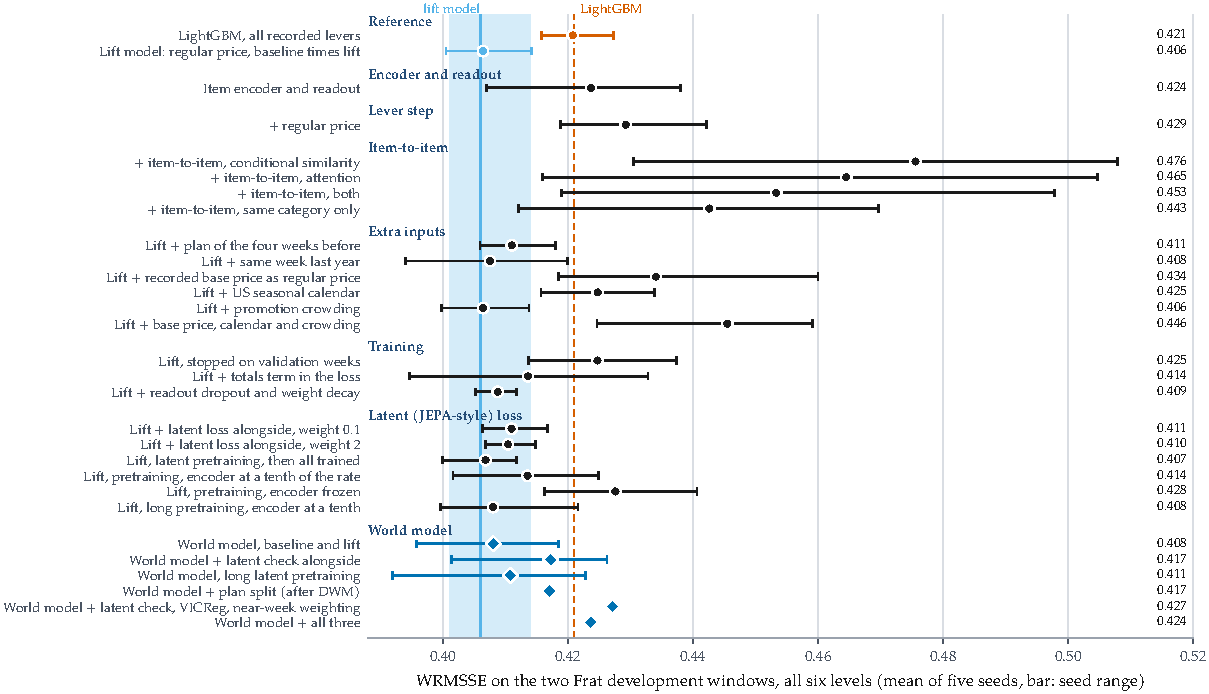
\includegraphics[width=\textwidth]{figs/fig_frat_dev.pdf}
\caption{\textbf{On Frat the gain came from building the forecast as a baseline
times a plan lift; item-to-item links, extra inputs, latent losses and the
roll-forward did not improve on it.} Each row is one configuration on the two
development windows, five seeds: mean (marker) and range (bar). Blue band: the
lift model's seed range; vertical lines: the lift model (0.406) and LightGBM
(0.421). Values below the lift model are in bold. Rows without a bar were
recorded as a mean only.}
\label{fig:fratdev}
\end{figure*}

\paragraph{What helped and what did not}
Figure~\ref{fig:fratdev} shows every configuration screened on Frat. Our item
encoder with a direct readout scored 0.424, level with LightGBM (0.421).
Building the forecast as a baseline under the nothing-planned plan times a lift
(the lift model) brought it to 0.406, better than LightGBM in all five runs and
with half the spread across seeds. Letting the 55 items in a store affect each
other, by conditional similarity, attention or both, made the forecast worse in
every version (0.443 to 0.476) and less steady; limiting it to items in the same
category narrowed the gap without closing it. Extra inputs did not help: the
plan of the four weeks before (0.411), the same week last year (0.408), the US
seasonal calendar (0.425), the count of items on promotion in the store (0.406)
and the recorded base price used as the regular price (0.434). The recorded
base price changes about twelve times a year per item and equals the shelf
price in every week without a promotion, so it is not a slow-moving regular
price.

\paragraph{Latent (JEPA-style) losses}
Following the JEPA literature~\cite{lecun2022,ijepa} and M-JEPA~\cite{mjepa}, we
added a loss that predicts the encoder's own state for the forecast weeks from
the state now and the plan, with a slowly updated copy of the encoder as the
target~\cite{byol}. No recipe beat the lift model: alongside the forecast loss
0.410 to 0.411, pretrained on the latent loss and then fine-tuned 0.407 to
0.414. With the encoder frozen after latent-only pretraining the model still
reached 0.428, so a state learned without any sales target carries most of the
forecast signal. Long pretraining followed by a slowed encoder gave the best
display-week error of any configuration (0.813 for the world model, against
0.817 for LightGBM).

\paragraph{The world model}
Rolling the state forward week by week under the plan scored 0.408, level with
the lift model on the overall score and on every lever. Three ideas from the
world-model literature, each at one untuned setting, did not help: keeping the
plan's effect apart from the no-plan state as in DWM~\cite{dwm} (0.417), a
latent check on each rolled step with a VICReg penalty~\cite{vicreg} and near
weeks weighted more as in TD-MPC2~\cite{tdmpc2} (0.427), and all three together
(0.424). Training changes did not help either: stopping at the best point on the
last 8 training weeks (0.425) took 8 of only 90 training weeks out of the
targets, and a term on summed totals in the loss (0.414) had no bias to fix,
since total forecasts were within 3\% of sales in every run. Readout dropout
with weight decay (0.409) was level and steadier, and was kept for the lift
model.

\input{generated/tab_tests}

\paragraph{Beyond accuracy}
Table~\ref{tab:tests} reports four further tests. \emph{New items}: with one
product in ten held out of training, the lift model borrowing the state and
level of the ten known items in the same store with the most labels in common
scored 0.890 on the new items, against 1.310 for LightGBM fitted on labels,
price and plan, and 1.510 for a forecast of zero. On Dominick's analgesics,
where items carry no category or maker labels, borrowing failed (2.999 against
0.923): the method needs item attributes. \emph{Combination}: weighting the lift
model and LightGBM on a validation window gave the best Frat result of the study
(0.388), better than either part on display and circular weeks, because the two
make different errors in promoted weeks; on analgesics the combination was
level. Combinations were not carried to the final tests, which compare single
models. \emph{Plan A against plan B}: for pairs of weeks of the same item and
store with different plans, every model picked the week that sold more about
78\% of the time; LightGBM was marginally ahead. \emph{Unusual plans}: on lever
mixes an item had run in under 2\% of its weeks, no model degraded much and
LightGBM stayed ahead. The world model's ability to roll a plan forward did not
show as an advantage on these tests.

\subsection{Dominick's}
\label{sec:dev-dom}

\paragraph{Analgesics, the category used to set the models}
On analgesics, seasonal naive scored 1.274, the average of the last 8 weeks
0.723 and LightGBM 0.715. The lift model scored 0.676 on three seeds, and the
world model 0.667 once a totals term was removed from its loss: that term made
the total worse, pulling forecasts 9\% low (0.819 for the lift model). Training
four times longer without a stop broke the summed levels (1.473) while
item-by-store error barely moved, so a small bias in the same direction on
every item added up at the category total. Five seeds changed the picture: the
world model held (0.666) and LightGBM scored 0.702, but the lift model fell to
0.718, so a three-seed figure had flattered it.

\begin{figure*}[t]
\centering
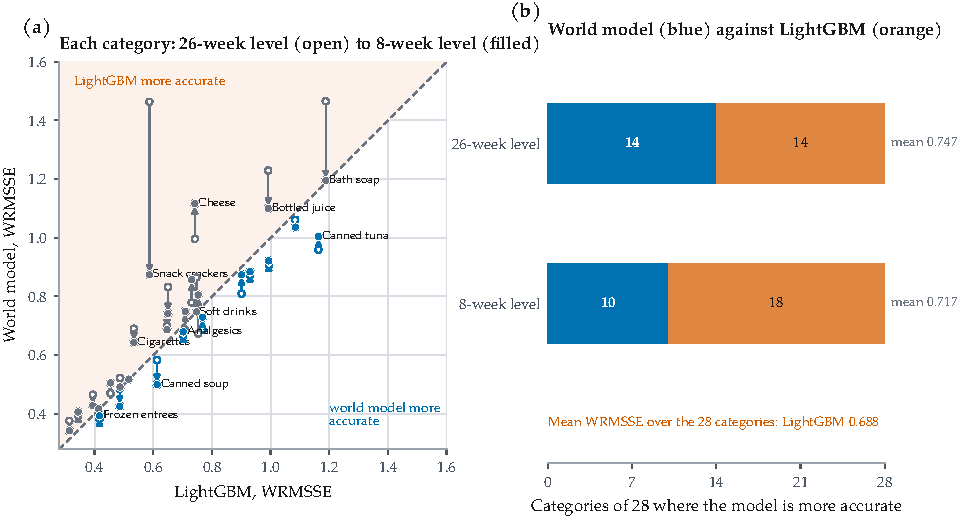
\includegraphics[width=\textwidth]{figs/fig_dom28.pdf}
\caption{\textbf{Run unchanged on all 28 Dominick's categories, the world model
set on analgesics failed badly in a few; taking each item's level from its last
8 weeks removed the worst failures but did not make it better than LightGBM on
average.} Development windows, one seed. \textbf{(a)} Each category's
WRMSSE for LightGBM (horizontal) and the world model (vertical), with the item
level from the last 26 weeks (open) and the last 8 weeks (filled); blue: the
world model is more accurate with the 8-week level. \textbf{(b)} Categories
where each model is more accurate, and the mean over the 28.}
\label{fig:dom28}
\end{figure*}

\paragraph{All 28 categories}
Run on all 28 categories with settings from analgesics, LightGBM was the most
accurate of the three in 14, the lift model in 5 and the world model in 9, with
mean WRMSSE 0.688, 0.784 and 0.747; on promoted weeks LightGBM was most accurate
in 24 of 27 (Figure~\ref{fig:dom28}, Table~\ref{tab:dom28}). Analgesics did not
generalise, which is why the paper reports every category. The failures (snack
crackers 1.463, bath soap 1.465, the lift model on soft drinks 1.406) sat at the
category total: item-by-store error was close to LightGBM's. On a six-store
sample of snack crackers the cause was in-and-out and seasonal lines: items
recorded in 8 to 20 of the last 26 weeks were 8\% of sales and the lift model
forecast them at 9 times their sales, because the model set each item's level from its 26-week
average after the item had fallen away. Capping extreme weeks did little; taking
the level from the last 8 weeks removed most of it. On all 28 categories the
8-week level brought the world model's mean to 0.717, removed the large failures
(snack crackers 1.463 to 0.874, bath soap 1.465 to 1.195) and gave a little back
in categories that had been fine, so it beat LightGBM in 10 categories against
14 before. LightGBM, which sees short recent averages directly, does not have the
problem.

\input{generated/tab_dom28}

\paragraph{Peaks and dips}
In cheese, both our model and LightGBM under-forecast promoted weeks by about a
third in the holiday window, and cheese peaks do not sit on a fixed week
relative to the holidays: they follow the chain's promotion timing, which event
flags cannot place. Figure~\ref{fig:peaks} splits forecast against sales into
promoted weeks, the weeks just after a promotion, and ordinary weeks, for six
categories. The world model did not see the dip after a promotion where the dip
is large: it forecast 1.33 times sales after a promotion in snack crackers and
1.32 in soft drinks, against 0.92 and 0.90 for LightGBM. Feeding the model's own
sales forecast into the roll-forward, so that a promotion's sales could shape the
weeks after it, fixed the soft-drink dip (1.32 to 1.00) and made the overall
score worse in four of six categories. Weighting the loss by dollar sales and by
how far a week sits from the item's usual level fixed cheese promoted weeks
(1.21 to 1.00) and was worse overall in three categories. In frozen entrees every
model, LightGBM included, forecast about 0.7 of sales after a promotion: there the
week after is stronger than any model expected.

\begin{figure*}[t]
\centering
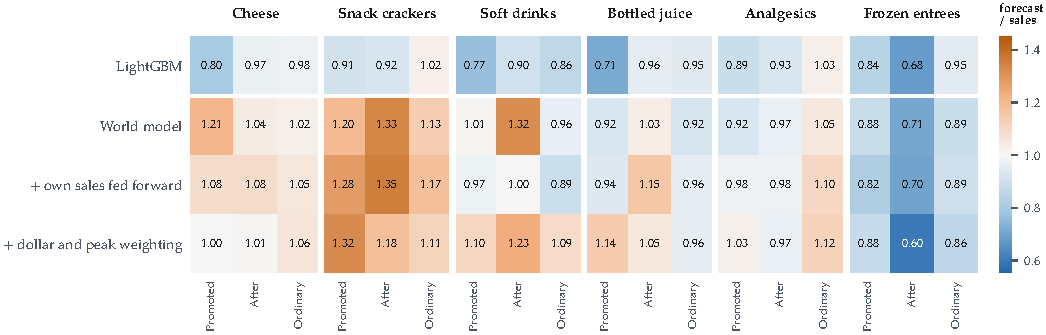
\includegraphics[width=\textwidth]{figs/fig_peaks.pdf}
\caption{\textbf{The world model over-forecast the weeks after a promotion where
shoppers had stocked up; the two fixes each repaired one category and hurt
others.} Forecast against sales (1.0 is right; orange over, blue under) in
promoted weeks, the weeks just after a promotion and ordinary weeks, Dominick's
development windows, one seed. Rows: LightGBM, the world model with the 8-week
level, with its own sales forecast fed forward, and with the loss weighted by
dollar sales and by peaks.}
\label{fig:peaks}
\end{figure*}

\paragraph{From the first world model to the one tested}
Figure~\ref{fig:ladder} follows the world model on the six categories through
the changes kept, three seeds each. Across seeds the first version was unsteady:
its range within a category was 0.04 to 0.38, against under 0.03 for LightGBM,
and on the mean LightGBM was ahead in five of six. Brand switching fixed what it
was built for: in snack crackers and soft drinks, where promoted weeks broke the
total, it was better on every seed (0.813 to 0.752, 0.902 to 0.789) and
item-by-store error improved too. The fitted share of the summed lift that the category total keeps
(Figure~\ref{fig:ladder}g) is 0.00 to 0.66 in snack crackers, against about 0.9
in bottled juice, analgesics and frozen entrees: in snack crackers the summed
item lifts overstated the category total, and the fit took most of it back.
Where it comes out at 1.0 the step changes nothing, a built-in check. The
direction agrees with van Heerde, Gupta and Wittink's household
estimates~\cite{vanheerde2003}, but the share is fitted to make totals right; it
is not an estimate of switching. Normalising the rolled state narrowed the seed range in five of six
categories, and averaging three fits per run with normalisation gave the
steadiest version (range 0.05 or less in five categories) and the candidate for
the final test: better than LightGBM on the three-seed mean in analgesics (0.622
against 0.701), frozen entrees (0.391 against 0.419) and soft drinks (0.743
against 0.759). One snack-cracker run of the three failed (1.806): its second
window's category total broke with promoted weeks forecast at 2.6 times sales
while item-by-store error stayed normal, so the summed promotion lift can still
run away on one fit in three. Twice the training steps, screened after the final
tests were fixed, was better in two categories, worse in two, level in one and
mixed in one, and was not kept.

\begin{figure*}[t]
\centering
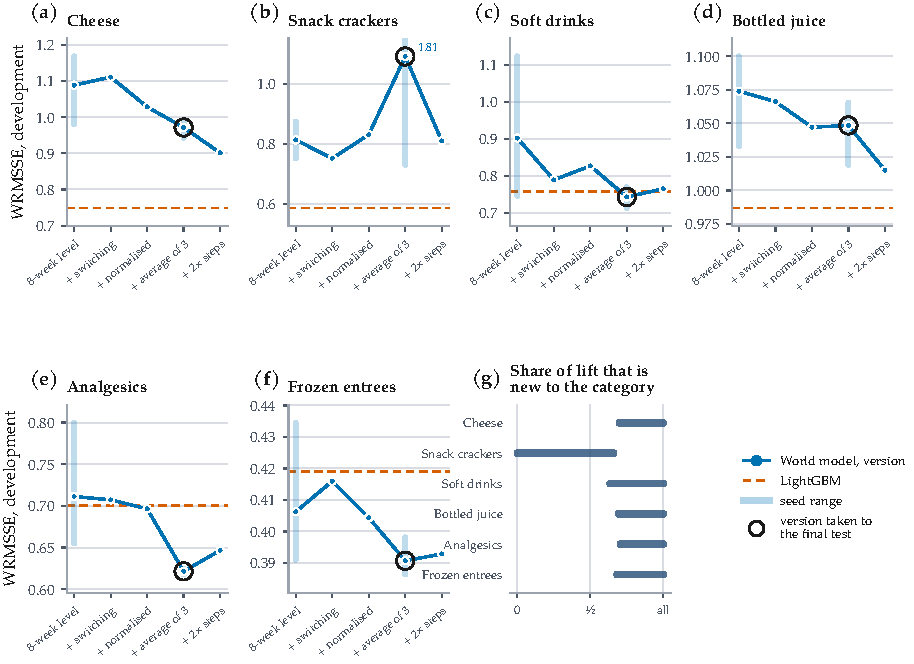
\includegraphics[width=\textwidth]{figs/fig_ladder.pdf}
\caption{\textbf{Brand switching, a normalised roll-forward and averaging three
fits took the world model past LightGBM in three of six categories on the
development windows, and the switching step learned how much of a promotion's
lift is new to the category.} \textbf{(a--f)} Development WRMSSE of each version,
three-seed means; shaded bars: seed range of the first version and of the one
taken to the final test (circled); dashed: LightGBM. \textbf{(g)} The fitted share of the summed promotion lift that the category
total keeps, the split that makes category totals fit best (not an estimate of
switching), range over runs.}
\label{fig:ladder}
\end{figure*}

\paragraph{Other changes}
Showing the model both its 26-week and its recent levels as inputs, instead of
setting its scale by the recent level, was the best world-model version in four
of ten categories but did not fix snack crackers (1.515) or soft drinks (1.069):
the model did not learn to switch to the recent level when the long level still
set its scale. Item role labels (new line, in-and-out, volume driver, long tail,
high-low, promotion-responsive, core), assigned from each item's own sales before
the windows, moved LightGBM by at most 0.013, since it reads the same information
from its history, and moved the world model in both directions; letting the role
pick the level broke snack crackers (2.422). We did not call the volume drivers
key value items, since a key-value-item list rests on shopper price perception,
which these data do not record.

\subsection{M5}
\label{sec:dev-m5}

\input{generated/tab_m5dev}

On the M5 practice window (Table~\ref{tab:m5dev}), the item encoder with a
direct readout scored 0.699 over five seeds against 0.715 for LightGBM, and the
lift and world models were level with LightGBM over three seeds (0.713 and
0.707). Normalising the rolled state was the one change that separated the world
model: 0.656, with its worst seed (0.675) better than the best seed without it
(0.680), all of the gain at the totals and the seed range cut from 0.070 to
0.029. It helped on M5's 28 daily steps and not on Dominick's 8 weekly steps,
which fits the reading that it stops the state drifting over a long roll.
Averaging three fits did not help on M5 (0.665), where single fits were already
steady.

After the official test month, an error analysis of the world model found its
2.6\% excess in Foods (+3.9\%), in one store (CA\_3, +7.5\%), and on Sundays and
Mondays (+5.1\%, +6.4\%), not growing with the horizon. Grouped by sales in the
28 days before the test, the excess came from items that had been selling fast
(+5.4\% and +6.1\% on items selling 3 to 10 and over 10 a day). Four changes
were screened on the practice window under rules written before screening:
weekday as seven inputs, event kinds, twice the training steps, and the item's
level against its past-year level. None beat the original
(Table~\ref{tab:m5dev}), so there was no second version. On the practice window
every version under-forecast by 4\% to 6\%, while on the test month the world
model over-forecast by 2.6\%: the sign of the level error changed between
adjacent months, so a fix tuned on one would not carry to the next. That
finding is what led to the confirmation months of \S\ref{sec:onemonth}.

% =====================================================================




\end{document}
